% Options for packages loaded elsewhere
\PassOptionsToPackage{unicode}{hyperref}
\PassOptionsToPackage{hyphens}{url}
\PassOptionsToPackage{dvipsnames,svgnames,x11names}{xcolor}
%
\documentclass[
  letterpaper,
  DIV=11,
  numbers=noendperiod]{scrartcl}

\usepackage{amsmath,amssymb}
\usepackage{iftex}
\ifPDFTeX
  \usepackage[T1]{fontenc}
  \usepackage[utf8]{inputenc}
  \usepackage{textcomp} % provide euro and other symbols
\else % if luatex or xetex
  \usepackage{unicode-math}
  \defaultfontfeatures{Scale=MatchLowercase}
  \defaultfontfeatures[\rmfamily]{Ligatures=TeX,Scale=1}
\fi
\usepackage{lmodern}
\ifPDFTeX\else  
    % xetex/luatex font selection
\fi
% Use upquote if available, for straight quotes in verbatim environments
\IfFileExists{upquote.sty}{\usepackage{upquote}}{}
\IfFileExists{microtype.sty}{% use microtype if available
  \usepackage[]{microtype}
  \UseMicrotypeSet[protrusion]{basicmath} % disable protrusion for tt fonts
}{}
\makeatletter
\@ifundefined{KOMAClassName}{% if non-KOMA class
  \IfFileExists{parskip.sty}{%
    \usepackage{parskip}
  }{% else
    \setlength{\parindent}{0pt}
    \setlength{\parskip}{6pt plus 2pt minus 1pt}}
}{% if KOMA class
  \KOMAoptions{parskip=half}}
\makeatother
\usepackage{xcolor}
\setlength{\emergencystretch}{3em} % prevent overfull lines
\setcounter{secnumdepth}{-\maxdimen} % remove section numbering
% Make \paragraph and \subparagraph free-standing
\makeatletter
\ifx\paragraph\undefined\else
  \let\oldparagraph\paragraph
  \renewcommand{\paragraph}{
    \@ifstar
      \xxxParagraphStar
      \xxxParagraphNoStar
  }
  \newcommand{\xxxParagraphStar}[1]{\oldparagraph*{#1}\mbox{}}
  \newcommand{\xxxParagraphNoStar}[1]{\oldparagraph{#1}\mbox{}}
\fi
\ifx\subparagraph\undefined\else
  \let\oldsubparagraph\subparagraph
  \renewcommand{\subparagraph}{
    \@ifstar
      \xxxSubParagraphStar
      \xxxSubParagraphNoStar
  }
  \newcommand{\xxxSubParagraphStar}[1]{\oldsubparagraph*{#1}\mbox{}}
  \newcommand{\xxxSubParagraphNoStar}[1]{\oldsubparagraph{#1}\mbox{}}
\fi
\makeatother

\usepackage{color}
\usepackage{fancyvrb}
\newcommand{\VerbBar}{|}
\newcommand{\VERB}{\Verb[commandchars=\\\{\}]}
\DefineVerbatimEnvironment{Highlighting}{Verbatim}{commandchars=\\\{\}}
% Add ',fontsize=\small' for more characters per line
\usepackage{framed}
\definecolor{shadecolor}{RGB}{241,243,245}
\newenvironment{Shaded}{\begin{snugshade}}{\end{snugshade}}
\newcommand{\AlertTok}[1]{\textcolor[rgb]{0.68,0.00,0.00}{#1}}
\newcommand{\AnnotationTok}[1]{\textcolor[rgb]{0.37,0.37,0.37}{#1}}
\newcommand{\AttributeTok}[1]{\textcolor[rgb]{0.40,0.45,0.13}{#1}}
\newcommand{\BaseNTok}[1]{\textcolor[rgb]{0.68,0.00,0.00}{#1}}
\newcommand{\BuiltInTok}[1]{\textcolor[rgb]{0.00,0.23,0.31}{#1}}
\newcommand{\CharTok}[1]{\textcolor[rgb]{0.13,0.47,0.30}{#1}}
\newcommand{\CommentTok}[1]{\textcolor[rgb]{0.37,0.37,0.37}{#1}}
\newcommand{\CommentVarTok}[1]{\textcolor[rgb]{0.37,0.37,0.37}{\textit{#1}}}
\newcommand{\ConstantTok}[1]{\textcolor[rgb]{0.56,0.35,0.01}{#1}}
\newcommand{\ControlFlowTok}[1]{\textcolor[rgb]{0.00,0.23,0.31}{\textbf{#1}}}
\newcommand{\DataTypeTok}[1]{\textcolor[rgb]{0.68,0.00,0.00}{#1}}
\newcommand{\DecValTok}[1]{\textcolor[rgb]{0.68,0.00,0.00}{#1}}
\newcommand{\DocumentationTok}[1]{\textcolor[rgb]{0.37,0.37,0.37}{\textit{#1}}}
\newcommand{\ErrorTok}[1]{\textcolor[rgb]{0.68,0.00,0.00}{#1}}
\newcommand{\ExtensionTok}[1]{\textcolor[rgb]{0.00,0.23,0.31}{#1}}
\newcommand{\FloatTok}[1]{\textcolor[rgb]{0.68,0.00,0.00}{#1}}
\newcommand{\FunctionTok}[1]{\textcolor[rgb]{0.28,0.35,0.67}{#1}}
\newcommand{\ImportTok}[1]{\textcolor[rgb]{0.00,0.46,0.62}{#1}}
\newcommand{\InformationTok}[1]{\textcolor[rgb]{0.37,0.37,0.37}{#1}}
\newcommand{\KeywordTok}[1]{\textcolor[rgb]{0.00,0.23,0.31}{\textbf{#1}}}
\newcommand{\NormalTok}[1]{\textcolor[rgb]{0.00,0.23,0.31}{#1}}
\newcommand{\OperatorTok}[1]{\textcolor[rgb]{0.37,0.37,0.37}{#1}}
\newcommand{\OtherTok}[1]{\textcolor[rgb]{0.00,0.23,0.31}{#1}}
\newcommand{\PreprocessorTok}[1]{\textcolor[rgb]{0.68,0.00,0.00}{#1}}
\newcommand{\RegionMarkerTok}[1]{\textcolor[rgb]{0.00,0.23,0.31}{#1}}
\newcommand{\SpecialCharTok}[1]{\textcolor[rgb]{0.37,0.37,0.37}{#1}}
\newcommand{\SpecialStringTok}[1]{\textcolor[rgb]{0.13,0.47,0.30}{#1}}
\newcommand{\StringTok}[1]{\textcolor[rgb]{0.13,0.47,0.30}{#1}}
\newcommand{\VariableTok}[1]{\textcolor[rgb]{0.07,0.07,0.07}{#1}}
\newcommand{\VerbatimStringTok}[1]{\textcolor[rgb]{0.13,0.47,0.30}{#1}}
\newcommand{\WarningTok}[1]{\textcolor[rgb]{0.37,0.37,0.37}{\textit{#1}}}

\providecommand{\tightlist}{%
  \setlength{\itemsep}{0pt}\setlength{\parskip}{0pt}}\usepackage{longtable,booktabs,array}
\usepackage{calc} % for calculating minipage widths
% Correct order of tables after \paragraph or \subparagraph
\usepackage{etoolbox}
\makeatletter
\patchcmd\longtable{\par}{\if@noskipsec\mbox{}\fi\par}{}{}
\makeatother
% Allow footnotes in longtable head/foot
\IfFileExists{footnotehyper.sty}{\usepackage{footnotehyper}}{\usepackage{footnote}}
\makesavenoteenv{longtable}
\usepackage{graphicx}
\makeatletter
\def\maxwidth{\ifdim\Gin@nat@width>\linewidth\linewidth\else\Gin@nat@width\fi}
\def\maxheight{\ifdim\Gin@nat@height>\textheight\textheight\else\Gin@nat@height\fi}
\makeatother
% Scale images if necessary, so that they will not overflow the page
% margins by default, and it is still possible to overwrite the defaults
% using explicit options in \includegraphics[width, height, ...]{}
\setkeys{Gin}{width=\maxwidth,height=\maxheight,keepaspectratio}
% Set default figure placement to htbp
\makeatletter
\def\fps@figure{htbp}
\makeatother

\usepackage{booktabs}
\usepackage{longtable}
\usepackage{array}
\usepackage{multirow}
\usepackage{wrapfig}
\usepackage{float}
\usepackage{colortbl}
\usepackage{pdflscape}
\usepackage{tabu}
\usepackage{threeparttable}
\usepackage{threeparttablex}
\usepackage[normalem]{ulem}
\usepackage{makecell}
\usepackage{xcolor}
\KOMAoption{captions}{tableheading}
\makeatletter
\@ifpackageloaded{caption}{}{\usepackage{caption}}
\AtBeginDocument{%
\ifdefined\contentsname
  \renewcommand*\contentsname{Table of contents}
\else
  \newcommand\contentsname{Table of contents}
\fi
\ifdefined\listfigurename
  \renewcommand*\listfigurename{List of Figures}
\else
  \newcommand\listfigurename{List of Figures}
\fi
\ifdefined\listtablename
  \renewcommand*\listtablename{List of Tables}
\else
  \newcommand\listtablename{List of Tables}
\fi
\ifdefined\figurename
  \renewcommand*\figurename{Figure}
\else
  \newcommand\figurename{Figure}
\fi
\ifdefined\tablename
  \renewcommand*\tablename{Table}
\else
  \newcommand\tablename{Table}
\fi
}
\@ifpackageloaded{float}{}{\usepackage{float}}
\floatstyle{ruled}
\@ifundefined{c@chapter}{\newfloat{codelisting}{h}{lop}}{\newfloat{codelisting}{h}{lop}[chapter]}
\floatname{codelisting}{Listing}
\newcommand*\listoflistings{\listof{codelisting}{List of Listings}}
\makeatother
\makeatletter
\makeatother
\makeatletter
\@ifpackageloaded{caption}{}{\usepackage{caption}}
\@ifpackageloaded{subcaption}{}{\usepackage{subcaption}}
\makeatother

\ifLuaTeX
  \usepackage{selnolig}  % disable illegal ligatures
\fi
\usepackage{bookmark}

\IfFileExists{xurl.sty}{\usepackage{xurl}}{} % add URL line breaks if available
\urlstyle{same} % disable monospaced font for URLs
\hypersetup{
  pdftitle={Rookie Contract Analysis},
  pdfauthor={Aidan McGrath, Ethan Martin, and Mitchell Darling},
  colorlinks=true,
  linkcolor={blue},
  filecolor={Maroon},
  citecolor={Blue},
  urlcolor={Blue},
  pdfcreator={LaTeX via pandoc}}


\title{Rookie Contract Analysis}
\author{Aidan McGrath, Ethan Martin, and Mitchell Darling}
\date{2025-05-07}

\begin{document}
\maketitle


\subsection{Overview}\label{overview}

The goal of our project is to see if there is a relation between an
athlete's performance during their rookie contract and how much their
next contract is worth. We are looking at the NHL, NBA, and NFL to see
if there are major differences between the leagues.

\subsection{NHL Data}\label{nhl-data}

The NHL's draft is different from other leagues because drafted players
often do not join their teams right away. This leads rookie contracts
for players drafted in the same year to not end at the same time. This
created some challenges because I could not simply merge a table of
players in a draft class with their statistics over the next three
seasons. I had to get data for different three season periods because of
this. This allowed me to merge players with the correct statistics for
their rookie contract.

The NHL player statistics were pulled from nhl.com using their export
feature. Their website allows users to filter statistics for players
drafted in certain drafts across specific seasons. They provide an
export button to export the filtered statistics into an excel file. The
contract data was taken from spotrac.com. There was no way to scrape the
data directly using R because there was not a page that had all of the
information I needed. I had to manually enter player's contract
information into an excel file that had the first 50 players drafted in
2015 and 2016. I then had to wrangle the data to remove cases that had
empty values. I was then able to merge the files together so every
player had their correct statistics for their rookie contract. This
resulted in each case being individual player.

This data adheres to CARE principles because all of the data I used is
publicly available and I gave credit to them. It also adheres to FAIR
principles because this data is easily found at the websites I
mentioned. I also used tidyverse to create the following data
visualizations.

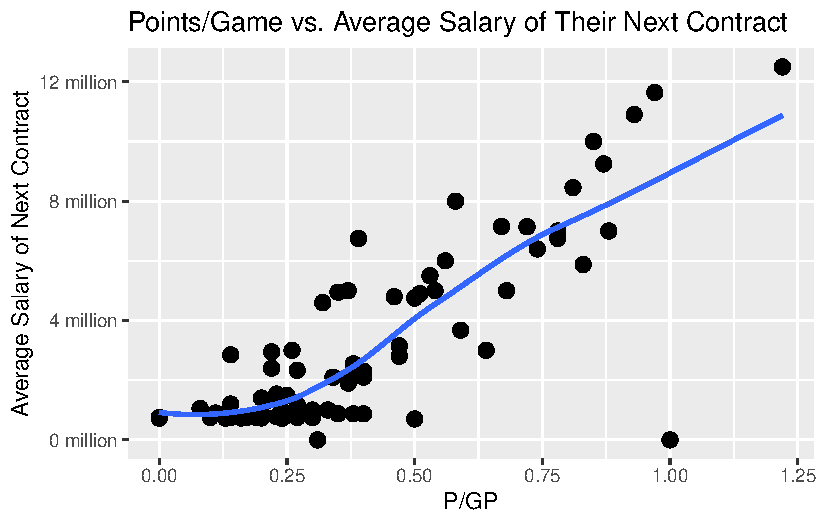
\includegraphics{final_qmd_file_files/figure-pdf/fig-NHL P/GP Graph-1.pdf}\{\#fig-NHL
P/GP Graph\}

This data visualization shows the relationship between a player's points
per game played and the average salary of of their next contract. In the
NHL, when a player scores a goal or assists on a goal they are awarded a
point. There is a clear relationship here that shows that the more
points per game played a player gets, the higher their next contract is
worth. There is an outlier in this data set where a player had 1 point
per game but did not receive a contract after their rookie contract
ended. This case is Egor Korshkov who decided to play in the Russian
league after his rookie contract was over.

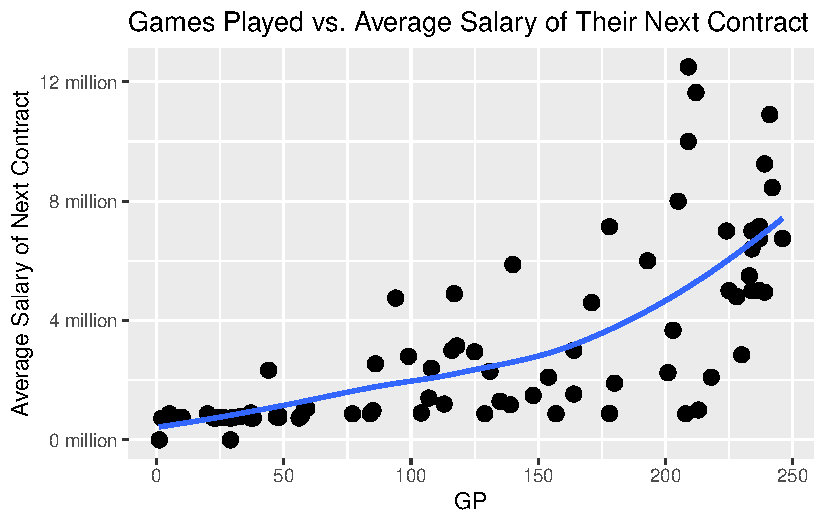
\includegraphics{final_qmd_file_files/figure-pdf/fig-NHL GP Graph-1.pdf}\{\#fig-NHL
GP Graph\}

This data visualization shows the relationship between games played
during a player's rookie contract and the average salary of their next
contract. There is still a relationship in this graph but it is not as
strong as the first one. This means that the strongest predictor for
average salary in the NHL is points per game played. This is an example
of exploratory data analysis because the goal of these visualizations is
to see if there are any relationships, not confirming a hypothesis.

\subsection{NBA Data}\label{nba-data}

\subsection{Three-Point Shooting vs
Salary}\label{three-point-shooting-vs-salary}

The NBA has been

\begin{Shaded}
\begin{Highlighting}[]
\FunctionTok{library}\NormalTok{(rvest)}
\FunctionTok{library}\NormalTok{(tidyverse)}
\FunctionTok{library}\NormalTok{(dplyr)}

\NormalTok{LeagueStatsWebPage }\OtherTok{\textless{}{-}} \FunctionTok{read\_html}\NormalTok{(}
  \StringTok{"https://www.basketball{-}reference.com/leagues/NBA\_stats\_per\_game.html\#stats{-}Regular{-}Season"}
\NormalTok{) }\SpecialCharTok{\%\textgreater{}\%} \FunctionTok{html\_elements}\NormalTok{(}\AttributeTok{css =} \StringTok{"table"}\NormalTok{) }\SpecialCharTok{\%\textgreater{}\%}
  \FunctionTok{html\_table}\NormalTok{()}

\NormalTok{LeagueStatsRaw }\OtherTok{\textless{}{-}}\NormalTok{ LeagueStatsWebPage[[}\DecValTok{1}\NormalTok{]]}

\CommentTok{\# Converts names of columns}
\FunctionTok{colnames}\NormalTok{(LeagueStatsRaw) }\OtherTok{\textless{}{-}} \FunctionTok{c}\NormalTok{(}\StringTok{"Rank"}\NormalTok{, }\StringTok{"Season"}\NormalTok{, }\StringTok{"Lg"}\NormalTok{, }\StringTok{"Age"}\NormalTok{, }\StringTok{"Height"}\NormalTok{, }\StringTok{"Weight"}\NormalTok{, }\StringTok{"Games"}\NormalTok{, }\StringTok{"MPG"}\NormalTok{, }\StringTok{"FGM"}\NormalTok{, }\StringTok{"FGA"}\NormalTok{, }\StringTok{"ThreePM"}\NormalTok{, }\StringTok{"ThreePA"}\NormalTok{, }\StringTok{"FT"}\NormalTok{, }\StringTok{"FTA"}\NormalTok{, }\StringTok{"ORB"}\NormalTok{, }\StringTok{"DRB"}\NormalTok{, }\StringTok{"TRB"}\NormalTok{, }\StringTok{"AST"}\NormalTok{, }\StringTok{"STL"}\NormalTok{, }\StringTok{"BLK"}\NormalTok{, }\StringTok{"TOV"}\NormalTok{, }\StringTok{"PF"}\NormalTok{, }\StringTok{"PTS"}\NormalTok{, }\StringTok{"FGPercent"}\NormalTok{, }\StringTok{"ThreePercent"}\NormalTok{, }\StringTok{"FTPercent"}\NormalTok{, }\StringTok{"Pace"}\NormalTok{, }\StringTok{"eFG\%"}\NormalTok{, }\StringTok{"TOVPercent"}\NormalTok{, }\StringTok{"ORBPercent"}\NormalTok{, }\StringTok{"FT/FGA"}\NormalTok{, }\StringTok{"ORtg"}\NormalTok{, }\StringTok{"TSPercent"}\NormalTok{)}

\CommentTok{\# Removes all but Year, 3PA, and 3P\%}

\CommentTok{\# Function to convert Season to Year format}
\NormalTok{convert\_year }\OtherTok{\textless{}{-}} \ControlFlowTok{function}\NormalTok{(year) \{}
\NormalTok{  yearEnd }\OtherTok{\textless{}{-}} \FunctionTok{substr}\NormalTok{(year, }\DecValTok{6}\NormalTok{, }\DecValTok{7}\NormalTok{)}
\NormalTok{  yearStart }\OtherTok{\textless{}{-}} \FunctionTok{substr}\NormalTok{(year, }\DecValTok{1}\NormalTok{, }\DecValTok{2}\NormalTok{)}
  \ControlFlowTok{if}\NormalTok{ (year }\SpecialCharTok{==} \StringTok{"1999{-}00"}\NormalTok{) \{}
\NormalTok{    newYear }\OtherTok{\textless{}{-}} \FunctionTok{paste}\NormalTok{(}\StringTok{"20"}\NormalTok{, }\AttributeTok{sep =} \StringTok{""}\NormalTok{, yearEnd)}
\NormalTok{  \} }\ControlFlowTok{else}\NormalTok{ \{}
\NormalTok{    newYear }\OtherTok{\textless{}{-}} \FunctionTok{paste}\NormalTok{(yearStart, }\AttributeTok{sep =} \StringTok{""}\NormalTok{, yearEnd)}
\NormalTok{  \}}
  \FunctionTok{return}\NormalTok{(newYear)}
\NormalTok{\}}

\CommentTok{\# Removes all but Year, 3PA, and 3P\% and removes leftover column name rows}
\NormalTok{LeagueStatsCleaned }\OtherTok{\textless{}{-}} \FunctionTok{select}\NormalTok{(LeagueStatsRaw, }\StringTok{"Season"}\NormalTok{, }\StringTok{"ThreePA"}\NormalTok{, }\StringTok{"ThreePercent"}\NormalTok{) }\SpecialCharTok{\%\textgreater{}\%}
  \FunctionTok{filter}\NormalTok{(Season }\SpecialCharTok{!=} \StringTok{"Season"}\NormalTok{) }\SpecialCharTok{\%\textgreater{}\%}
  \FunctionTok{filter}\NormalTok{(ThreePercent }\SpecialCharTok{!=} \StringTok{"Shooting"}\NormalTok{) }\SpecialCharTok{\%\textgreater{}\%}
  \FunctionTok{rowwise}\NormalTok{() }\SpecialCharTok{\%\textgreater{}\%}
  \FunctionTok{mutate}\NormalTok{(}
    \AttributeTok{Year =} \FunctionTok{convert\_year}\NormalTok{(Season)}
\NormalTok{  ) }\SpecialCharTok{\%\textgreater{}\%}
  \FunctionTok{filter}\NormalTok{(Season }\SpecialCharTok{\textgreater{}} \DecValTok{1979}\NormalTok{)}

\NormalTok{LeagueStatsCleaned }\OtherTok{\textless{}{-}} \FunctionTok{mutate}\NormalTok{(LeagueStatsCleaned, }\AttributeTok{ThreePA =} \FunctionTok{as.numeric}\NormalTok{(ThreePA))}
\NormalTok{LeagueStatsCleaned }\OtherTok{\textless{}{-}} \FunctionTok{mutate}\NormalTok{(LeagueStatsCleaned, }\AttributeTok{Year =} \FunctionTok{as.numeric}\NormalTok{(Year))}

\FunctionTok{ggplot}\NormalTok{(}
  \AttributeTok{data =}\NormalTok{ LeagueStatsCleaned,}
  \AttributeTok{mapping =} \FunctionTok{aes}\NormalTok{(}
  \AttributeTok{x =}\NormalTok{ Year,}
  \AttributeTok{y =}\NormalTok{ ThreePA}
\NormalTok{  )}
\NormalTok{) }\SpecialCharTok{+} \FunctionTok{geom\_line}\NormalTok{() }\SpecialCharTok{+}
  \FunctionTok{theme\_bw}\NormalTok{() }\SpecialCharTok{+}
  \FunctionTok{labs}\NormalTok{(}
    \AttributeTok{x =} \StringTok{\textquotesingle{}Year\textquotesingle{}}\NormalTok{,}
    \AttributeTok{y =} \StringTok{\textquotesingle{}Three Pointers Attempted Per Game\textquotesingle{}}
\NormalTok{  )}
\end{Highlighting}
\end{Shaded}

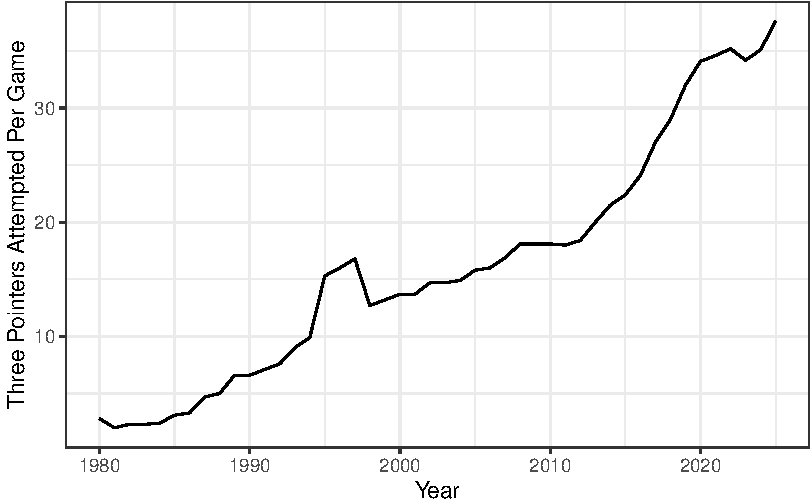
\includegraphics{final_qmd_file_files/figure-pdf/unnamed-chunk-1-1.pdf}

\subsection{NFL Data}\label{nfl-data}

This section focuses on data from the NFL. This ranges from the draft
data, to contract/salary information, to player statistics throughout
the duration of the season. I aim to perform an EDA based approach on
these datasets in order to identify what factors play into the value of
a player's contract, whether that be draft pick positioning, college
career stats, production in the league, or any other factor that becomes
relevant when discussing a player's paycheck. Specifically, I will be
focusing on data from the 2020 NFL Draft class. This gives me a 5-year
period (seasons 2020-2024) to study and evaluate the performance of new
players. In an attempt to isolate variables and factors that will play
into how a player is payed, I am focusing my analysis to offensive
players. Specifically what are called ``Skill Position'' players. These
are offensive players that score touchdowns: Quarterback (QB), running
back (RB), wide receiver (WR), and tight end (TE). However, I will be
omitting the tight end position from the majority of analyses due to
variations in data, as the tight end position's purpose isn't just to
score points. They are often used as a power back, a blocker, and then
also a receiver to catch passes, so due to the varied nature of this
position, I won't be using it when evaluating scoring statistics.

The NFL uses position abbreviations in order to simplify names and
reduce space taken up, and so have I. So for those unaware of football
argon, here are what each position abbreviation means:

C -- Center, CB -- Corner Back (Often grouped with safeties as DB), ED
-- Edge, FB -- Full Back, IDL -- Interior Defensive Lineman, K --
Kicker, LB -- Linebacker, LG -- Left Guard, LS -- Long Snapper, LT --
Left Tackle, P -- Punter, QB -- Quarterback, RB -- Running Back, RG --
Right Guard, RT -- Right Tackle, S -- Safety, TE -- Tight End, WR --
Wide Receiver.

The data is sourced from various sites, but the majority is from
websites like Pro Football Reference and Spotrac, two sites that
prioritize accurate, free, and public records of anything NFL related.
Draft stats, team stats, stat leaders, and any other statistic of the
sort that pertains to NFL football can be found on these sites and are
commonly cross referenced and used by professional sport analysts
nationwide. I used Pro Football Reference for the 2020 NFL Draft order
and the college career stats of the players selected in said draft year.
Spotrac was used for contract information, mainly for salary extensions
throughout the specified time period. I also used an r package called
``nflreadr'', which had more useful information about contract periods
and player salary.

\begin{figure}[H]

\centering{

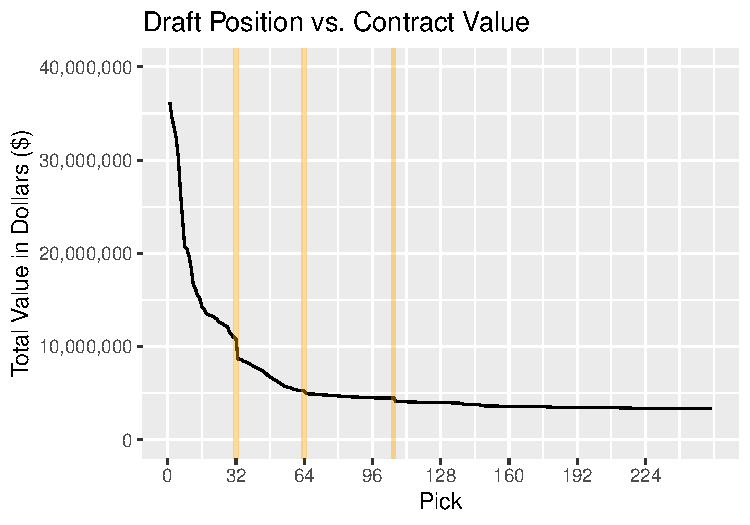
\includegraphics{final_qmd_file_files/figure-pdf/fig-contract_signing_scale-1.pdf}

}

\caption{\label{fig-contract_signing_scale}Scale of Contract Value
vs.~Draft Pick}

\end{figure}%

The graph above is a typical line graph of the rookie contract value of
all players drafted in the 2020 NFL draft. The draft is split into 7, 32
pick rounds, but this number isnt always firm due to forfeiture and
compensatory picks. But the first and second round all experience a
significant drop in salary value upon their conclusion, while the drop
decreases steadily as the draft progresses. This graph has a few
vertical lines to isolate the first, second, and third rounds. We can
pick out from this graph that the NFL (and their teams) all prioritize
and dump as much money as they can into the first round of the draft, as
this is when the best players end up getting drafted. This is one of the
few solid factors that are directly related to a player's contract
value.

\begin{figure}[H]

\centering{

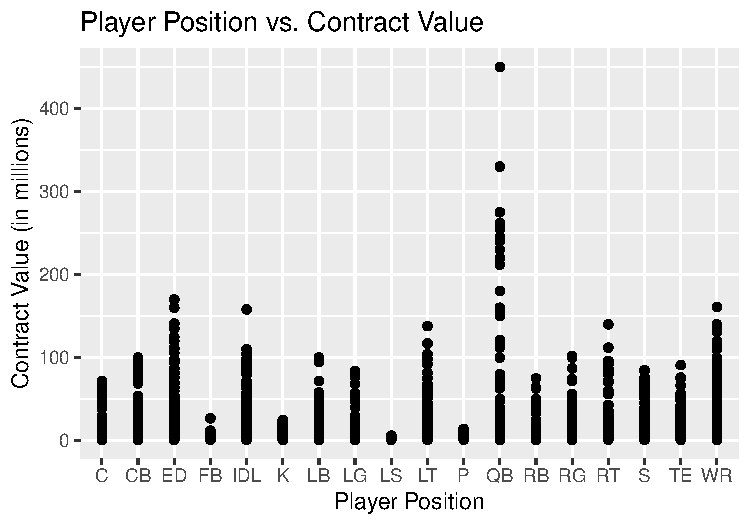
\includegraphics{final_qmd_file_files/figure-pdf/fig-pos_vs_contract-1.pdf}

}

\caption{\label{fig-pos_vs_contract}Position vs.~Contract Value by
Position}

\end{figure}%

This is a grouped scatter plot, grouped by player position, where each
case is an individual player and their contract. If the position names
at the bottom are still a little confusing, please refer to the key
stated in the NFL section's introduction. Not much can be gained from
this graph, or a visualization of any sort based upon this dataset due
to its scattered and varied nature, however, we do see that the
Quarterback position, by far, has the highest value associated with it.
Which makes sense when we consider that the quarterback is the only
player (aside from the center, who starts the play) who handles the
football every single play. They also are the primary point scorers, as
they throw the ball to the receivers (which counts as a score for both
players, statistic-wise), and can also run the ball to score. Coming up
next behind the QB position is the edge rushers, followed by wide
receivers. Edge rushers value comes from their ability to pressure the
quarterback and halt run plays, making them incredibly valuable on
defense. As for the receivers, they bring the bag home in regards to how
necessary they are for a high powered offense to score. They create
threats down the field and open the play up, again, making them a highly
sought after asset.

\begin{figure}[H]

\centering{

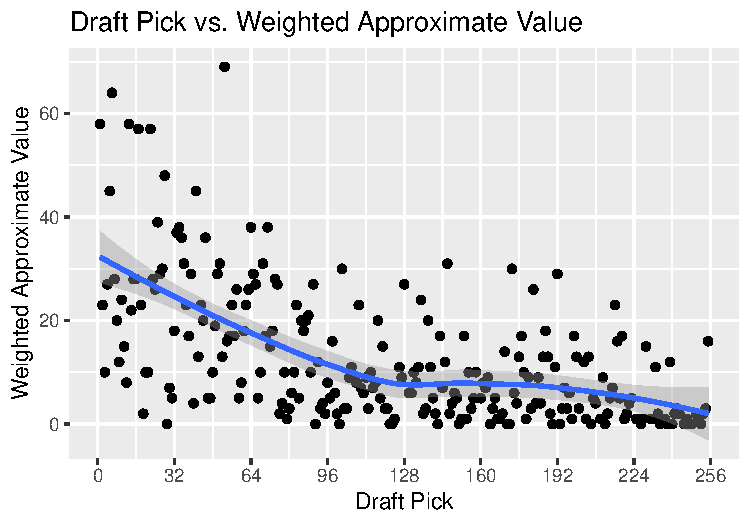
\includegraphics{final_qmd_file_files/figure-pdf/fig-pick_vs_weighted_approx_value-1.pdf}

}

\caption{\label{fig-pick_vs_weighted_approx_value}Draft Pick
vs.~Weighted Approximate Value}

\end{figure}%

This visualization explores the affect of WAV (wighted approximate
value). WAV is a statistic used to evaluate a college football player's
overall ``value'' or contribution to the team. This statistic varies
across different positions and rarely is a determining factor in where
and when a player gets drafted. It is solely a number that a draftee or
college player is given that corresponds to their ``seasonal value''.
Here we can see that the higher WAV players do tend to get drafted
earlier, but that observation only holds true in the earlier rounds of
the draft. After the third round (usually around pick 96) we can see
that higher WAV does not relate to the position the draftee is taken. I
have added a trend line to help visualize variations in this graph but
it proves the point that WAV does not play a meaningful factor in the
outcome of a player's draft spot.

\begin{figure}[H]

\centering{

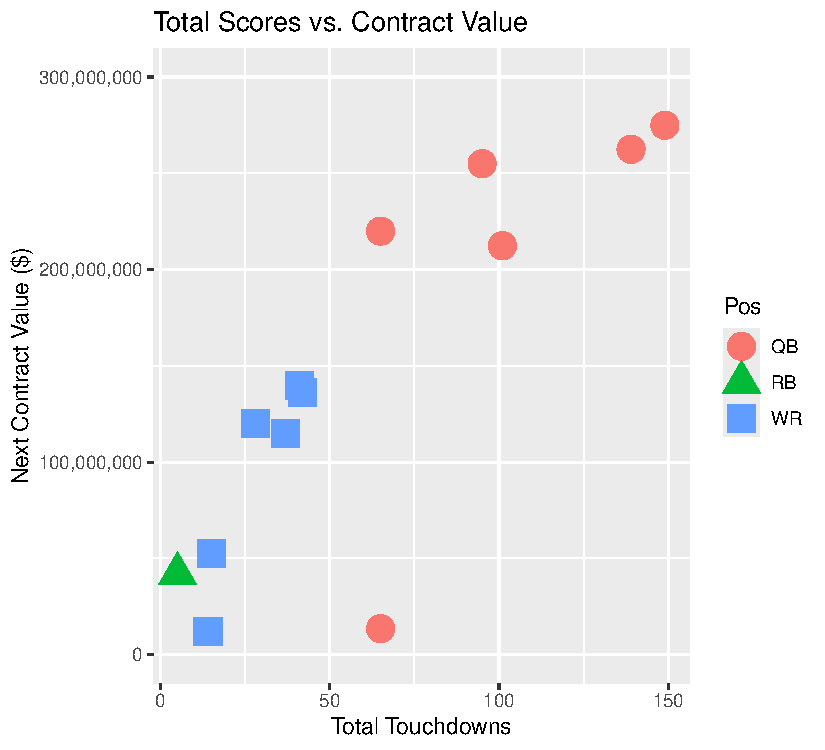
\includegraphics{final_qmd_file_files/figure-pdf/fig-scores_vs_salary-1.pdf}

}

\caption{\label{fig-scores_vs_salary}Number of Touchdowns vs.~Salary by
Position}

\end{figure}%

Context for this graph: this is data that has been extensively filtered
to match specific cases I wanted to isolate. Unlike other visualizations
that utilized the entire set of data, I filtered these only to match
players who have signed a contract extension sometime after their
initial draft in 2020. In other words, these are players that make it
through the jump to the professional level of the sport. So, due to
these conditions (skill positions minus TE, drafted in 2020, and
re-signed sometime before 2025) the sample size for this visualization
is small, but provides solid cases that should help in further analysis.

This is a visualization that attempts to put the skill positions on a
common, level playing field, that is the total amount of scores
(touchdowns) they achieve. However, this ``even playing field'' is about
as even and level as the Rocky Mountains, as not every skill position
scores as often as the others do. But, there is still important
information we can extract from this visualization. We can see that the
successful QBs in this plot both score and are paid more than their
offensive counterparts, both WRs and RBs.

\begin{table}[H]

\caption{\label{tbl-dollar_per_score}Dollar Per Score By Skill Position}

\centering{

\begin{tabu} to \linewidth {>{\raggedright}X>{\raggedright}X>{\raggedright}X>{\raggedright}X}
\toprule
Pos & Touchdowns & Total Salary & Dollars per Touchdown\\
\midrule
QB & 614  (77.14\%) & 1,238,400,000  (66.73\%) & 2,016,938  (14.76\%)\\
RB & 5   (0.63\%) & 42,000,000   (2.26\%) & 8,400,000  (61.46\%)\\
WR & 177  (22.24\%) & 575,390,000  (31.01\%) & 3,250,791  (23.78\%)\\
Total & 796 (100.00\%) & 1,855,790,000 (100.00\%) & 13,667,729 (100.00\%)\\
\bottomrule
\end{tabu}

}

\end{table}%

This is a summary table based upon the visualization above
(Figure~\ref{fig-scores_vs_salary}). Using the same sample size, we can
look at the makeup of their salaries, total touchdowns, and the relation
between them. QBs are scoring the vast majority of touchdowns, making up
more than three quarters of the sample data. However, this table breeds
a very important relation that is applicable across all point scorers,
which is Dollars per Touchdown. QBs, on average, will make about 2
million dollars per touchdown they score, and WRs about 3 and a quarter
million per score. But RBs get a little interesting. The running back
position in the NFL has been a very controversial position in regards to
payment. They are the most injury-prone, and have some of the lowest pay
in the league for their troubles. Consulting the Position vs.~Salary
graph (Figure~\ref{fig-pos_vs_contract}), we can see that they have some
of the lowest median and mean pay for their position group. However,
when evaluated along the same criteria I have been using, we can see
that they will be paid a whopping 8.4 million per touchdown that they
score. So we see here that RBs might not score the most often or get
paid frequently, but when they score, it is apparent that it means a lot
more in terms of monetary value.

\subsection{Comparing Sports}\label{comparing-sports}

All three leagues we looked at have at least one player statistic that
has a strong relationship with the average salary of their next
contract. This shows that it is possible to predict the value of a
player's contract only with one or two statistics. This is important to
recognize for players so they can ensure they are being paid adequately.

For the NFL, the main factors that play into a rookie player's salary
and contract value are draft positioning, and if they are a point scorer
or not. Draft positioning (Figure~\ref{fig-contract_signing_scale})
proves the first point among what factors affect a player's contract
value. The second, according to player position
(Figure~\ref{fig-pos_vs_contract}), that we see is that point scorers,
especially quarterbacks, get the bag at an incredibly disproportionate
level.

For the NFL, the main factors that play into a rookie player's salary
and contract value are draft positioning, and if they are a point scorer
or not. Draft positioning from the draft position vs.~contract graph
proves the first point among what factors affect a player's contract
value. The second, according to the position vs.~contract grouped plot,
that we see is that point scorers, especially quarterbacks, get the bag
at an incredibly disproportionate level.

For the NHL, the main factor that impacted a player's salary was points
per game. This makes sense because if a player is scoring or assisting a
lot, they are valuable and teams will want to keep them. This makes the
team willing to pay them more. Another factor that impacted a player's
salary was games played. This also makes sense because if a coach is
choosing to play someone, it is likely because they are good which means
they get paid more.

After comparison between all three sports, we can identify that the one
commonality is how they score. Whether its points per game or
touchdowns, the main idea is if you score you get paid. As much as draft
``stock'' and positioning play into a player's initial rookie contract,
their prolonged success (and consequently payment and contract value) is
determined by how efficient they are at scoring.

\subsection{Citations}\label{citations}

``Statistics.'' NHL.Com, www.nhl.com/stats/. Accessed 7 May 2025.

NHL \textbar{} Spotrac.Com, www.spotrac.com/nhl. Accessed 8 May 2025.

``NFL Contract Extensions.'' Spotrac.Com,
www.spotrac.com/nfl/contracts/extensions. Accessed 8 May 2025.

``2020 NFL Draft Listing.'' Pro Football Reference,
www.pro-football-reference.com/years/2020/draft.html. Accessed 7 May
2025.

``NFLREADR • Download NFLVERSE Data.'' NFLreadr, nflreadr.nflverse.com/.
Accessed 7 May 2025.

\subsection{Code Apendix}\label{code-apendix}

\begin{Shaded}
\begin{Highlighting}[]
\CommentTok{\#loading the necessary packages}
\FunctionTok{library}\NormalTok{(tidyverse)}
\FunctionTok{library}\NormalTok{(rvest)}
\FunctionTok{library}\NormalTok{(dplyr)}
\FunctionTok{library}\NormalTok{(ggplot2)}
\FunctionTok{library}\NormalTok{(readxl)}

\CommentTok{\#importing data}
\NormalTok{nhl\_draft\_2015 }\OtherTok{\textless{}{-}} \FunctionTok{read\_excel}\NormalTok{(}
  \StringTok{"/Users/ethanmartin/Downloads/nhl\_draft\_2015.xlsx"}
\NormalTok{  )}
\NormalTok{nhl\_draft\_2016 }\OtherTok{\textless{}{-}} \FunctionTok{read\_excel}\NormalTok{(}
  \StringTok{"/Users/ethanmartin/Downloads/nhl\_draft\_2016.xlsx"}
\NormalTok{  )}
\NormalTok{rookies\_2015\_to\_2017 }\OtherTok{\textless{}{-}} \FunctionTok{read\_excel}\NormalTok{(}
  \StringTok{"/Users/ethanmartin/Downloads/rookies\_2015\_to\_2017.xlsx"}
\NormalTok{  )}
\NormalTok{rookies\_2015\_to\_2018 }\OtherTok{\textless{}{-}} \FunctionTok{read\_excel}\NormalTok{(}
  \StringTok{"/Users/ethanmartin/Downloads/rookies\_2015\_to\_2018.xlsx"}
\NormalTok{  )}
\NormalTok{rookies\_2015\_to\_2019 }\OtherTok{\textless{}{-}} \FunctionTok{read\_excel}\NormalTok{(}
  \StringTok{"/Users/ethanmartin/Downloads/rookies\_2015\_to\_2019.xlsx"}
\NormalTok{  )}
\NormalTok{rookies\_2015\_to\_2020 }\OtherTok{\textless{}{-}} \FunctionTok{read\_excel}\NormalTok{(}
  \StringTok{"/Users/ethanmartin/Downloads/rookies\_2015\_to\_2020.xlsx"}
\NormalTok{  )}
\NormalTok{rookies\_2016\_to\_2018 }\OtherTok{\textless{}{-}} \FunctionTok{read\_excel}\NormalTok{(}
  \StringTok{"/Users/ethanmartin/Downloads/rookies\_2016\_to\_2018.xlsx"}
\NormalTok{  )}
\NormalTok{rookies\_2016\_to\_2019 }\OtherTok{\textless{}{-}} \FunctionTok{read\_excel}\NormalTok{(}
  \StringTok{"/Users/ethanmartin/Downloads/rookies\_2016\_to\_2019.xlsx"}
\NormalTok{  )}
\NormalTok{rookies\_2016\_to\_2020 }\OtherTok{\textless{}{-}} \FunctionTok{read\_excel}\NormalTok{(}
  \StringTok{"/Users/ethanmartin/Downloads/rookies\_2016\_to\_2020.xlsx"}
\NormalTok{  )}
\NormalTok{rookies\_2016\_to\_2021 }\OtherTok{\textless{}{-}} \FunctionTok{read\_excel}\NormalTok{(}
  \StringTok{"/Users/ethanmartin/Downloads/rookies\_2016\_to\_2021.xlsx"}
\NormalTok{  )}

\CommentTok{\#filtering the data}
\NormalTok{rookies2015to2017 }\OtherTok{\textless{}{-}}\NormalTok{ nhl\_draft\_2015 }\SpecialCharTok{\%\textgreater{}\%}
  \FunctionTok{filter}\NormalTok{(}\StringTok{\textasciigrave{}}\AttributeTok{End of Rookie Contract}\StringTok{\textasciigrave{}} \SpecialCharTok{==} \DecValTok{2017}\NormalTok{)}

\NormalTok{rookies2015to2018 }\OtherTok{\textless{}{-}}\NormalTok{ nhl\_draft\_2015 }\SpecialCharTok{\%\textgreater{}\%}
  \FunctionTok{filter}\NormalTok{(}\StringTok{\textasciigrave{}}\AttributeTok{End of Rookie Contract}\StringTok{\textasciigrave{}} \SpecialCharTok{==} \DecValTok{2018}\NormalTok{)}

\NormalTok{rookies2015to2019 }\OtherTok{\textless{}{-}}\NormalTok{ nhl\_draft\_2015 }\SpecialCharTok{\%\textgreater{}\%}
  \FunctionTok{filter}\NormalTok{(}\StringTok{\textasciigrave{}}\AttributeTok{End of Rookie Contract}\StringTok{\textasciigrave{}} \SpecialCharTok{==} \DecValTok{2019}\NormalTok{)}

\NormalTok{rookies2015to2020 }\OtherTok{\textless{}{-}}\NormalTok{ nhl\_draft\_2015 }\SpecialCharTok{\%\textgreater{}\%}
  \FunctionTok{filter}\NormalTok{(}\StringTok{\textasciigrave{}}\AttributeTok{End of Rookie Contract}\StringTok{\textasciigrave{}} \SpecialCharTok{==} \DecValTok{2020}\NormalTok{)}

\NormalTok{rookies2016to2018 }\OtherTok{\textless{}{-}}\NormalTok{ nhl\_draft\_2016 }\SpecialCharTok{\%\textgreater{}\%}
  \FunctionTok{filter}\NormalTok{(}\StringTok{\textasciigrave{}}\AttributeTok{End of Rookie Contract}\StringTok{\textasciigrave{}} \SpecialCharTok{==} \DecValTok{2018}\NormalTok{)}

\NormalTok{rookies2016to2019 }\OtherTok{\textless{}{-}}\NormalTok{ nhl\_draft\_2016 }\SpecialCharTok{\%\textgreater{}\%}
  \FunctionTok{filter}\NormalTok{(}\StringTok{\textasciigrave{}}\AttributeTok{End of Rookie Contract}\StringTok{\textasciigrave{}} \SpecialCharTok{==} \DecValTok{2019}\NormalTok{)}

\NormalTok{rookies2016to2020 }\OtherTok{\textless{}{-}}\NormalTok{ nhl\_draft\_2016 }\SpecialCharTok{\%\textgreater{}\%}
  \FunctionTok{filter}\NormalTok{(}\StringTok{\textasciigrave{}}\AttributeTok{End of Rookie Contract}\StringTok{\textasciigrave{}} \SpecialCharTok{==} \DecValTok{2020}\NormalTok{)}

\NormalTok{rookies2016to2021 }\OtherTok{\textless{}{-}}\NormalTok{ nhl\_draft\_2016 }\SpecialCharTok{\%\textgreater{}\%}
  \FunctionTok{filter}\NormalTok{(}\StringTok{\textasciigrave{}}\AttributeTok{End of Rookie Contract}\StringTok{\textasciigrave{}} \SpecialCharTok{==} \DecValTok{2021}\NormalTok{)}

\CommentTok{\#merges the filtered data with player stats}
\NormalTok{rookieStats2015to2017 }\OtherTok{\textless{}{-}} \FunctionTok{left\_join}\NormalTok{(}
  \AttributeTok{x =}\NormalTok{ rookies2015to2017,}
  \AttributeTok{y =}\NormalTok{ rookies\_2015\_to\_2017,}
  \AttributeTok{by =} \FunctionTok{join\_by}\NormalTok{(Player }\SpecialCharTok{==}\NormalTok{ Player)}
\NormalTok{) }\SpecialCharTok{\%\textgreater{}\%}
  \FunctionTok{drop\_na}\NormalTok{() }\SpecialCharTok{\%\textgreater{}\%}
  \FunctionTok{mutate}\NormalTok{(}\AttributeTok{S =} \FunctionTok{as.numeric}\NormalTok{(S))}

\NormalTok{rookieStats2015to2018 }\OtherTok{\textless{}{-}} \FunctionTok{left\_join}\NormalTok{(}
  \AttributeTok{x =}\NormalTok{ rookies2015to2018,}
  \AttributeTok{y =}\NormalTok{ rookies\_2015\_to\_2018,}
  \AttributeTok{by =} \FunctionTok{join\_by}\NormalTok{(Player }\SpecialCharTok{==}\NormalTok{ Player)}
\NormalTok{) }\SpecialCharTok{\%\textgreater{}\%}
  \FunctionTok{drop\_na}\NormalTok{() }\SpecialCharTok{\%\textgreater{}\%}
  \FunctionTok{mutate}\NormalTok{(}\AttributeTok{S =} \FunctionTok{as.numeric}\NormalTok{(S))}

\NormalTok{rookieStats2015to2019 }\OtherTok{\textless{}{-}} \FunctionTok{left\_join}\NormalTok{(}
  \AttributeTok{x =}\NormalTok{ rookies2015to2019,}
  \AttributeTok{y =}\NormalTok{ rookies\_2015\_to\_2019,}
  \AttributeTok{by =} \FunctionTok{join\_by}\NormalTok{(Player }\SpecialCharTok{==}\NormalTok{ Player)}
\NormalTok{) }\SpecialCharTok{\%\textgreater{}\%}
  \FunctionTok{drop\_na}\NormalTok{() }\SpecialCharTok{\%\textgreater{}\%}
  \FunctionTok{mutate}\NormalTok{(}\AttributeTok{S =} \FunctionTok{as.numeric}\NormalTok{(S))}

\NormalTok{rookieStats2015to2020 }\OtherTok{\textless{}{-}} \FunctionTok{left\_join}\NormalTok{(}
  \AttributeTok{x =}\NormalTok{ rookies2015to2020,}
  \AttributeTok{y =}\NormalTok{ rookies\_2015\_to\_2020,}
  \AttributeTok{by =} \FunctionTok{join\_by}\NormalTok{(Player }\SpecialCharTok{==}\NormalTok{ Player)}
\NormalTok{) }\SpecialCharTok{\%\textgreater{}\%}
  \FunctionTok{drop\_na}\NormalTok{() }\SpecialCharTok{\%\textgreater{}\%}
  \FunctionTok{mutate}\NormalTok{(}\AttributeTok{S =} \FunctionTok{as.numeric}\NormalTok{(S))}

\NormalTok{rookieStats2016to2018 }\OtherTok{\textless{}{-}} \FunctionTok{left\_join}\NormalTok{(}
  \AttributeTok{x =}\NormalTok{ rookies2016to2018,}
  \AttributeTok{y =}\NormalTok{ rookies\_2016\_to\_2018,}
  \AttributeTok{by =} \FunctionTok{join\_by}\NormalTok{(Player }\SpecialCharTok{==}\NormalTok{ Player)}
\NormalTok{) }\SpecialCharTok{\%\textgreater{}\%}
  \FunctionTok{drop\_na}\NormalTok{() }\SpecialCharTok{\%\textgreater{}\%}
  \FunctionTok{mutate}\NormalTok{(}\AttributeTok{S =} \FunctionTok{as.numeric}\NormalTok{(S))}

\NormalTok{rookieStats2016to2019 }\OtherTok{\textless{}{-}} \FunctionTok{left\_join}\NormalTok{(}
  \AttributeTok{x =}\NormalTok{ rookies2016to2019,}
  \AttributeTok{y =}\NormalTok{ rookies\_2016\_to\_2019,}
  \AttributeTok{by =} \FunctionTok{join\_by}\NormalTok{(Player }\SpecialCharTok{==}\NormalTok{ Player)}
\NormalTok{) }\SpecialCharTok{\%\textgreater{}\%}
  \FunctionTok{drop\_na}\NormalTok{() }\SpecialCharTok{\%\textgreater{}\%}
  \FunctionTok{mutate}\NormalTok{(}\AttributeTok{S =} \FunctionTok{as.numeric}\NormalTok{(S))}

\NormalTok{rookieStats2016to2020 }\OtherTok{\textless{}{-}} \FunctionTok{left\_join}\NormalTok{(}
  \AttributeTok{x =}\NormalTok{ rookies2016to2020,}
  \AttributeTok{y =}\NormalTok{ rookies\_2016\_to\_2020,}
  \AttributeTok{by =} \FunctionTok{join\_by}\NormalTok{(Player }\SpecialCharTok{==}\NormalTok{ Player)}
\NormalTok{) }\SpecialCharTok{\%\textgreater{}\%}
  \FunctionTok{drop\_na}\NormalTok{() }\SpecialCharTok{\%\textgreater{}\%}
  \FunctionTok{mutate}\NormalTok{(}\AttributeTok{S =} \FunctionTok{as.numeric}\NormalTok{(S))}

\NormalTok{rookieStats2016to2021 }\OtherTok{\textless{}{-}} \FunctionTok{left\_join}\NormalTok{(}
  \AttributeTok{x =}\NormalTok{ rookies2016to2021,}
  \AttributeTok{y =}\NormalTok{ rookies\_2016\_to\_2021,}
  \AttributeTok{by =} \FunctionTok{join\_by}\NormalTok{(Player }\SpecialCharTok{==}\NormalTok{ Player)}
\NormalTok{) }\SpecialCharTok{\%\textgreater{}\%}
  \FunctionTok{drop\_na}\NormalTok{() }\SpecialCharTok{\%\textgreater{}\%}
  \FunctionTok{mutate}\NormalTok{(}\AttributeTok{S =} \FunctionTok{as.numeric}\NormalTok{(S))}

\CommentTok{\#combines all data sets and generalizes the positions }
\NormalTok{all\_rookie\_stats }\OtherTok{\textless{}{-}} \FunctionTok{bind\_rows}\NormalTok{(}
\NormalTok{  rookieStats2015to2017,}
\NormalTok{  rookieStats2015to2018,}
\NormalTok{  rookieStats2015to2019,}
\NormalTok{  rookieStats2015to2020,}
\NormalTok{  rookieStats2016to2018,}
\NormalTok{  rookieStats2016to2019,}
\NormalTok{  rookieStats2016to2020,}
\NormalTok{  rookieStats2016to2021}
\NormalTok{) }\SpecialCharTok{\%\textgreater{}\%}
  \FunctionTok{select}\NormalTok{(}\SpecialCharTok{{-}}\NormalTok{Pos) }\SpecialCharTok{\%\textgreater{}\%}
  \FunctionTok{mutate}\NormalTok{(}\AttributeTok{Position =} \FunctionTok{ifelse}\NormalTok{(Position }\SpecialCharTok{==} \StringTok{"C"}\NormalTok{, }\StringTok{"Forward"}\NormalTok{, Position)) }\SpecialCharTok{\%\textgreater{}\%}
  \FunctionTok{mutate}\NormalTok{(}\AttributeTok{Position =} \FunctionTok{ifelse}\NormalTok{(Position }\SpecialCharTok{==} \StringTok{"LW"}\NormalTok{, }\StringTok{"Forward"}\NormalTok{, Position)) }\SpecialCharTok{\%\textgreater{}\%}
  \FunctionTok{mutate}\NormalTok{(}\AttributeTok{Position =} \FunctionTok{ifelse}\NormalTok{(Position }\SpecialCharTok{==} \StringTok{"RW"}\NormalTok{, }\StringTok{"Forward"}\NormalTok{, Position)) }\SpecialCharTok{\%\textgreater{}\%}
  \FunctionTok{mutate}\NormalTok{(}\AttributeTok{Position =} \FunctionTok{ifelse}\NormalTok{(Position }\SpecialCharTok{==} \StringTok{"D"}\NormalTok{, }\StringTok{"Defenseman"}\NormalTok{, Position))}

\CommentTok{\#creates points per game graph}
\NormalTok{ppg\_graph }\OtherTok{\textless{}{-}} \FunctionTok{ggplot}\NormalTok{(}
\NormalTok{  all\_rookie\_stats, }\FunctionTok{aes}\NormalTok{(}\AttributeTok{x =} \StringTok{\textasciigrave{}}\AttributeTok{P/GP}\StringTok{\textasciigrave{}}\NormalTok{, }\AttributeTok{y =} \StringTok{\textasciigrave{}}\AttributeTok{Average Salary of Next Contract}\StringTok{\textasciigrave{}}\NormalTok{)}
\NormalTok{  ) }\SpecialCharTok{+}
  \FunctionTok{geom\_point}\NormalTok{(}\AttributeTok{size =} \DecValTok{3}\NormalTok{) }\SpecialCharTok{+}
  \FunctionTok{geom\_smooth}\NormalTok{(}\AttributeTok{method =} \StringTok{"loess"}\NormalTok{, }\AttributeTok{se =} \ConstantTok{FALSE}\NormalTok{) }\SpecialCharTok{+}
  \FunctionTok{scale\_y\_continuous}\NormalTok{(}\AttributeTok{labels =} \ControlFlowTok{function}\NormalTok{(x) }\FunctionTok{paste0}\NormalTok{(x }\SpecialCharTok{/} \FloatTok{1e6}\NormalTok{, }\StringTok{" million"}\NormalTok{)) }\SpecialCharTok{+}
  \FunctionTok{labs}\NormalTok{(}
    \AttributeTok{title =} \StringTok{"Points/Game vs. Average Salary of Their Next Contract"}
\NormalTok{  )}

\CommentTok{\#creates games played graph}
\NormalTok{gp\_graph }\OtherTok{\textless{}{-}} \FunctionTok{ggplot}\NormalTok{(all\_rookie\_stats, }\FunctionTok{aes}\NormalTok{(}
  \AttributeTok{x =} \StringTok{\textasciigrave{}}\AttributeTok{GP}\StringTok{\textasciigrave{}}\NormalTok{, }\AttributeTok{y =} \StringTok{\textasciigrave{}}\AttributeTok{Average Salary of Next Contract}\StringTok{\textasciigrave{}}\NormalTok{)}
\NormalTok{  ) }\SpecialCharTok{+}
  \FunctionTok{geom\_point}\NormalTok{(}\AttributeTok{size =} \DecValTok{3}\NormalTok{) }\SpecialCharTok{+}
  \FunctionTok{geom\_smooth}\NormalTok{(}\AttributeTok{method =} \StringTok{"loess"}\NormalTok{, }\AttributeTok{se =} \ConstantTok{FALSE}\NormalTok{) }\SpecialCharTok{+}
  \FunctionTok{scale\_y\_continuous}\NormalTok{(}\AttributeTok{labels =} \ControlFlowTok{function}\NormalTok{(x) }\FunctionTok{paste0}\NormalTok{(x }\SpecialCharTok{/} \FloatTok{1e6}\NormalTok{, }\StringTok{" million"}\NormalTok{)) }\SpecialCharTok{+}
  \FunctionTok{labs}\NormalTok{(}
    \AttributeTok{title =} \StringTok{"Games Played vs. Average Salary of Their Next Contract"}
\NormalTok{  )}
\NormalTok{ppg\_graph}
\NormalTok{gp\_graph}
\FunctionTok{library}\NormalTok{(rvest)}
\FunctionTok{library}\NormalTok{(tidyverse)}
\FunctionTok{library}\NormalTok{(dplyr)}

\NormalTok{LeagueStatsWebPage }\OtherTok{\textless{}{-}} \FunctionTok{read\_html}\NormalTok{(}
  \StringTok{"https://www.basketball{-}reference.com/leagues/NBA\_stats\_per\_game.html\#stats{-}Regular{-}Season"}
\NormalTok{) }\SpecialCharTok{\%\textgreater{}\%} \FunctionTok{html\_elements}\NormalTok{(}\AttributeTok{css =} \StringTok{"table"}\NormalTok{) }\SpecialCharTok{\%\textgreater{}\%}
  \FunctionTok{html\_table}\NormalTok{()}

\NormalTok{LeagueStatsRaw }\OtherTok{\textless{}{-}}\NormalTok{ LeagueStatsWebPage[[}\DecValTok{1}\NormalTok{]]}

\CommentTok{\# Converts names of columns}
\FunctionTok{colnames}\NormalTok{(LeagueStatsRaw) }\OtherTok{\textless{}{-}} \FunctionTok{c}\NormalTok{(}\StringTok{"Rank"}\NormalTok{, }\StringTok{"Season"}\NormalTok{, }\StringTok{"Lg"}\NormalTok{, }\StringTok{"Age"}\NormalTok{, }\StringTok{"Height"}\NormalTok{, }\StringTok{"Weight"}\NormalTok{, }\StringTok{"Games"}\NormalTok{, }\StringTok{"MPG"}\NormalTok{, }\StringTok{"FGM"}\NormalTok{, }\StringTok{"FGA"}\NormalTok{, }\StringTok{"ThreePM"}\NormalTok{, }\StringTok{"ThreePA"}\NormalTok{, }\StringTok{"FT"}\NormalTok{, }\StringTok{"FTA"}\NormalTok{, }\StringTok{"ORB"}\NormalTok{, }\StringTok{"DRB"}\NormalTok{, }\StringTok{"TRB"}\NormalTok{, }\StringTok{"AST"}\NormalTok{, }\StringTok{"STL"}\NormalTok{, }\StringTok{"BLK"}\NormalTok{, }\StringTok{"TOV"}\NormalTok{, }\StringTok{"PF"}\NormalTok{, }\StringTok{"PTS"}\NormalTok{, }\StringTok{"FGPercent"}\NormalTok{, }\StringTok{"ThreePercent"}\NormalTok{, }\StringTok{"FTPercent"}\NormalTok{, }\StringTok{"Pace"}\NormalTok{, }\StringTok{"eFG\%"}\NormalTok{, }\StringTok{"TOVPercent"}\NormalTok{, }\StringTok{"ORBPercent"}\NormalTok{, }\StringTok{"FT/FGA"}\NormalTok{, }\StringTok{"ORtg"}\NormalTok{, }\StringTok{"TSPercent"}\NormalTok{)}

\CommentTok{\# Removes all but Year, 3PA, and 3P\%}

\CommentTok{\# Function to convert Season to Year format}
\NormalTok{convert\_year }\OtherTok{\textless{}{-}} \ControlFlowTok{function}\NormalTok{(year) \{}
\NormalTok{  yearEnd }\OtherTok{\textless{}{-}} \FunctionTok{substr}\NormalTok{(year, }\DecValTok{6}\NormalTok{, }\DecValTok{7}\NormalTok{)}
\NormalTok{  yearStart }\OtherTok{\textless{}{-}} \FunctionTok{substr}\NormalTok{(year, }\DecValTok{1}\NormalTok{, }\DecValTok{2}\NormalTok{)}
  \ControlFlowTok{if}\NormalTok{ (year }\SpecialCharTok{==} \StringTok{"1999{-}00"}\NormalTok{) \{}
\NormalTok{    newYear }\OtherTok{\textless{}{-}} \FunctionTok{paste}\NormalTok{(}\StringTok{"20"}\NormalTok{, }\AttributeTok{sep =} \StringTok{""}\NormalTok{, yearEnd)}
\NormalTok{  \} }\ControlFlowTok{else}\NormalTok{ \{}
\NormalTok{    newYear }\OtherTok{\textless{}{-}} \FunctionTok{paste}\NormalTok{(yearStart, }\AttributeTok{sep =} \StringTok{""}\NormalTok{, yearEnd)}
\NormalTok{  \}}
  \FunctionTok{return}\NormalTok{(newYear)}
\NormalTok{\}}

\CommentTok{\# Removes all but Year, 3PA, and 3P\% and removes leftover column name rows}
\NormalTok{LeagueStatsCleaned }\OtherTok{\textless{}{-}} \FunctionTok{select}\NormalTok{(LeagueStatsRaw, }\StringTok{"Season"}\NormalTok{, }\StringTok{"ThreePA"}\NormalTok{, }\StringTok{"ThreePercent"}\NormalTok{) }\SpecialCharTok{\%\textgreater{}\%}
  \FunctionTok{filter}\NormalTok{(Season }\SpecialCharTok{!=} \StringTok{"Season"}\NormalTok{) }\SpecialCharTok{\%\textgreater{}\%}
  \FunctionTok{filter}\NormalTok{(ThreePercent }\SpecialCharTok{!=} \StringTok{"Shooting"}\NormalTok{) }\SpecialCharTok{\%\textgreater{}\%}
  \FunctionTok{rowwise}\NormalTok{() }\SpecialCharTok{\%\textgreater{}\%}
  \FunctionTok{mutate}\NormalTok{(}
    \AttributeTok{Year =} \FunctionTok{convert\_year}\NormalTok{(Season)}
\NormalTok{  ) }\SpecialCharTok{\%\textgreater{}\%}
  \FunctionTok{filter}\NormalTok{(Season }\SpecialCharTok{\textgreater{}} \DecValTok{1979}\NormalTok{)}

\NormalTok{LeagueStatsCleaned }\OtherTok{\textless{}{-}} \FunctionTok{mutate}\NormalTok{(LeagueStatsCleaned, }\AttributeTok{ThreePA =} \FunctionTok{as.numeric}\NormalTok{(ThreePA))}
\NormalTok{LeagueStatsCleaned }\OtherTok{\textless{}{-}} \FunctionTok{mutate}\NormalTok{(LeagueStatsCleaned, }\AttributeTok{Year =} \FunctionTok{as.numeric}\NormalTok{(Year))}

\FunctionTok{ggplot}\NormalTok{(}
  \AttributeTok{data =}\NormalTok{ LeagueStatsCleaned,}
  \AttributeTok{mapping =} \FunctionTok{aes}\NormalTok{(}
  \AttributeTok{x =}\NormalTok{ Year,}
  \AttributeTok{y =}\NormalTok{ ThreePA}
\NormalTok{  )}
\NormalTok{) }\SpecialCharTok{+} \FunctionTok{geom\_line}\NormalTok{() }\SpecialCharTok{+}
  \FunctionTok{theme\_bw}\NormalTok{() }\SpecialCharTok{+}
  \FunctionTok{labs}\NormalTok{(}
    \AttributeTok{x =} \StringTok{\textquotesingle{}Year\textquotesingle{}}\NormalTok{,}
    \AttributeTok{y =} \StringTok{\textquotesingle{}Three Pointers Attempted Per Game\textquotesingle{}}
\NormalTok{  )}

\CommentTok{\# Packages {-}{-}{-}{-}}
\CommentTok{\# install.packages("rvest")}
\CommentTok{\# install.packages("tidyverse")}
\CommentTok{\# install.packages("googlesheets4")}
\CommentTok{\# install.packages("nflreadr")}
\CommentTok{\# install.packages("ggplot2")}
\CommentTok{\# install.packages("dplyr")}
\CommentTok{\# install.packages("hrbrthemes")}
\CommentTok{\# install.packages("viridis")}
\CommentTok{\# install.packages("janitor")}
\CommentTok{\# install.packages("knitr")}
\CommentTok{\# install.packages("kableExtra")}
\CommentTok{\# install.packages("ggpmisc")}
\CommentTok{\# install.packages("tinytex")}
\FunctionTok{library}\NormalTok{(nflreadr)}
\FunctionTok{library}\NormalTok{(rvest)}
\FunctionTok{library}\NormalTok{(tidyverse)}
\FunctionTok{library}\NormalTok{(googlesheets4)}
\FunctionTok{library}\NormalTok{(ggplot2)}
\FunctionTok{library}\NormalTok{(dplyr)}
\FunctionTok{library}\NormalTok{(hrbrthemes)}
\FunctionTok{library}\NormalTok{(viridis)}
\FunctionTok{library}\NormalTok{(data.table)}
\FunctionTok{library}\NormalTok{(janitor)}
\FunctionTok{library}\NormalTok{(knitr)}
\FunctionTok{library}\NormalTok{(kableExtra)}
\FunctionTok{library}\NormalTok{(ggpmisc)}
\FunctionTok{library}\NormalTok{(tinytex)}
\FunctionTok{library}\NormalTok{(chromote)}

\CommentTok{\# Scraping {-}{-}{-}{-}}
\CommentTok{\# NFL signing and salary table }
\NormalTok{nfl\_salary\_raw }\OtherTok{\textless{}{-}} \FunctionTok{read\_html\_live}\NormalTok{(}\StringTok{"https://www.spotrac.com/nfl/contracts"}\NormalTok{) }\SpecialCharTok{\%\textgreater{}\%}
  \FunctionTok{html\_elements}\NormalTok{(}\AttributeTok{css =} \StringTok{"table"}\NormalTok{) }\SpecialCharTok{\%\textgreater{}\%}
  \FunctionTok{html\_table}\NormalTok{()}
\NormalTok{nfl\_salary }\OtherTok{\textless{}{-}}\NormalTok{ nfl\_salary\_raw[[}\DecValTok{2}\NormalTok{]]}

\CommentTok{\# NFL contract extensions since 2021}
\NormalTok{extensions\_2021\_raw }\OtherTok{\textless{}{-}} \FunctionTok{read\_html\_live}\NormalTok{(}\StringTok{"https://www.spotrac.com/nfl/contracts/extensions/\_/year/2021"}\NormalTok{) }\SpecialCharTok{\%\textgreater{}\%}
  \FunctionTok{html\_elements}\NormalTok{(}\AttributeTok{css =} \StringTok{"table"}\NormalTok{) }\SpecialCharTok{\%\textgreater{}\%}
  \FunctionTok{html\_table}\NormalTok{()}
\NormalTok{extensions\_2021 }\OtherTok{\textless{}{-}}\NormalTok{ extensions\_2021\_raw[[}\DecValTok{2}\NormalTok{]]}

\NormalTok{extensions\_2022\_raw }\OtherTok{\textless{}{-}} \FunctionTok{read\_html\_live}\NormalTok{(}\StringTok{"https://www.spotrac.com/nfl/contracts/extensions/\_/year/2022/"}\NormalTok{) }\SpecialCharTok{\%\textgreater{}\%}
  \FunctionTok{html\_elements}\NormalTok{(}\AttributeTok{css =} \StringTok{"table"}\NormalTok{) }\SpecialCharTok{\%\textgreater{}\%}
  \FunctionTok{html\_table}\NormalTok{()}
\NormalTok{extensions\_2022 }\OtherTok{\textless{}{-}}\NormalTok{ extensions\_2022\_raw[[}\DecValTok{2}\NormalTok{]]}

\NormalTok{extensions\_2023\_raw }\OtherTok{\textless{}{-}} \FunctionTok{read\_html\_live}\NormalTok{(}\StringTok{"https://www.spotrac.com/nfl/contracts/extensions/\_/year/2023/"}\NormalTok{) }\SpecialCharTok{\%\textgreater{}\%}
  \FunctionTok{html\_elements}\NormalTok{(}\AttributeTok{css =} \StringTok{"table"}\NormalTok{) }\SpecialCharTok{\%\textgreater{}\%}
  \FunctionTok{html\_table}\NormalTok{()}
\NormalTok{extensions\_2023 }\OtherTok{\textless{}{-}}\NormalTok{ extensions\_2023\_raw[[}\DecValTok{2}\NormalTok{]]}

\NormalTok{extensions\_2024\_raw }\OtherTok{\textless{}{-}} \FunctionTok{read\_html\_live}\NormalTok{(}\StringTok{"https://www.spotrac.com/nfl/contracts/extensions/\_/year/2024/"}\NormalTok{) }\SpecialCharTok{\%\textgreater{}\%}
  \FunctionTok{html\_elements}\NormalTok{(}\AttributeTok{css =} \StringTok{"table"}\NormalTok{) }\SpecialCharTok{\%\textgreater{}\%}
  \FunctionTok{html\_table}\NormalTok{()}
\NormalTok{extensions\_2024 }\OtherTok{\textless{}{-}}\NormalTok{ extensions\_2024\_raw[[}\DecValTok{2}\NormalTok{]]}

\NormalTok{extensions\_2025\_raw }\OtherTok{\textless{}{-}} \FunctionTok{read\_html\_live}\NormalTok{(}\StringTok{"https://www.spotrac.com/nfl/contracts/extensions/\_/year/2025/"}\NormalTok{) }\SpecialCharTok{\%\textgreater{}\%}
  \FunctionTok{html\_elements}\NormalTok{(}\AttributeTok{css =} \StringTok{"table"}\NormalTok{) }\SpecialCharTok{\%\textgreater{}\%}
  \FunctionTok{html\_table}\NormalTok{()}
\NormalTok{extensions\_2025 }\OtherTok{\textless{}{-}}\NormalTok{ extensions\_2025\_raw[[}\DecValTok{2}\NormalTok{]]}
\FunctionTok{names}\NormalTok{(extensions\_2021)[}\DecValTok{2}\NormalTok{] }\OtherTok{\textless{}{-}} \StringTok{"Player"}
\FunctionTok{names}\NormalTok{(extensions\_2022)[}\DecValTok{2}\NormalTok{] }\OtherTok{\textless{}{-}} \StringTok{"Player"}
\FunctionTok{names}\NormalTok{(extensions\_2023)[}\DecValTok{2}\NormalTok{] }\OtherTok{\textless{}{-}} \StringTok{"Player"}
\FunctionTok{names}\NormalTok{(extensions\_2024)[}\DecValTok{2}\NormalTok{] }\OtherTok{\textless{}{-}} \StringTok{"Player"}
\FunctionTok{names}\NormalTok{(extensions\_2025)[}\DecValTok{2}\NormalTok{] }\OtherTok{\textless{}{-}} \StringTok{"Player"}
\NormalTok{extensions\_all }\OtherTok{\textless{}{-}} \FunctionTok{bind\_rows}\NormalTok{(}
  \FunctionTok{list}\NormalTok{(extensions\_2021, extensions\_2022, extensions\_2023, extensions\_2024, extensions\_2025)}
\NormalTok{)}
\CommentTok{\# NFL rookie contract "signing scale" for the 2020 draft year by pick}
\NormalTok{rookie\_scale\_raw }\OtherTok{\textless{}{-}} \FunctionTok{read\_html\_live}\NormalTok{(}\StringTok{"https://www.spotrac.com/nfl/cba/rookie{-}scale/\_/year/2020"}\NormalTok{) }\SpecialCharTok{\%\textgreater{}\%}
  \FunctionTok{html\_elements}\NormalTok{(}\AttributeTok{css =} \StringTok{"table"}\NormalTok{) }\SpecialCharTok{\%\textgreater{}\%}
  \FunctionTok{html\_table}\NormalTok{()}
\NormalTok{rookie\_scale }\OtherTok{\textless{}{-}}\NormalTok{ rookie\_scale\_raw[[}\DecValTok{1}\NormalTok{]]}
\NormalTok{rookie\_scale}\SpecialCharTok{$}\StringTok{\textasciigrave{}}\AttributeTok{Total Value}\StringTok{\textasciigrave{}} \OtherTok{=} \FunctionTok{as.numeric}\NormalTok{(}\FunctionTok{gsub}\NormalTok{(}\StringTok{"[}\SpecialCharTok{\textbackslash{}\textbackslash{}}\StringTok{$,]"}\NormalTok{,}\StringTok{""}\NormalTok{, rookie\_scale}\SpecialCharTok{$}\StringTok{\textasciigrave{}}\AttributeTok{Total Value}\StringTok{\textasciigrave{}}\NormalTok{))}
\NormalTok{rookie\_scale}\SpecialCharTok{$}\StringTok{\textasciigrave{}}\AttributeTok{Year 1}\StringTok{\textasciigrave{}} \OtherTok{=} \FunctionTok{as.numeric}\NormalTok{(}\FunctionTok{gsub}\NormalTok{(}\StringTok{"[}\SpecialCharTok{\textbackslash{}\textbackslash{}}\StringTok{$,]"}\NormalTok{,}\StringTok{""}\NormalTok{, rookie\_scale}\SpecialCharTok{$}\StringTok{\textasciigrave{}}\AttributeTok{Year 1}\StringTok{\textasciigrave{}}\NormalTok{))}
\NormalTok{rookie\_scale}\SpecialCharTok{$}\StringTok{\textasciigrave{}}\AttributeTok{Year 2}\StringTok{\textasciigrave{}} \OtherTok{=} \FunctionTok{as.numeric}\NormalTok{(}\FunctionTok{gsub}\NormalTok{(}\StringTok{"[}\SpecialCharTok{\textbackslash{}\textbackslash{}}\StringTok{$,]"}\NormalTok{,}\StringTok{""}\NormalTok{, rookie\_scale}\SpecialCharTok{$}\StringTok{\textasciigrave{}}\AttributeTok{Year 2}\StringTok{\textasciigrave{}}\NormalTok{))}
\NormalTok{rookie\_scale}\SpecialCharTok{$}\StringTok{\textasciigrave{}}\AttributeTok{Year 3}\StringTok{\textasciigrave{}} \OtherTok{=} \FunctionTok{as.numeric}\NormalTok{(}\FunctionTok{gsub}\NormalTok{(}\StringTok{"[}\SpecialCharTok{\textbackslash{}\textbackslash{}}\StringTok{$,]"}\NormalTok{,}\StringTok{""}\NormalTok{, rookie\_scale}\SpecialCharTok{$}\StringTok{\textasciigrave{}}\AttributeTok{Year 3}\StringTok{\textasciigrave{}}\NormalTok{))}
\NormalTok{rookie\_scale}\SpecialCharTok{$}\StringTok{\textasciigrave{}}\AttributeTok{Year 4}\StringTok{\textasciigrave{}} \OtherTok{=} \FunctionTok{as.numeric}\NormalTok{(}\FunctionTok{gsub}\NormalTok{(}\StringTok{"[}\SpecialCharTok{\textbackslash{}\textbackslash{}}\StringTok{$,]"}\NormalTok{,}\StringTok{""}\NormalTok{, rookie\_scale}\SpecialCharTok{$}\StringTok{\textasciigrave{}}\AttributeTok{Year 4}\StringTok{\textasciigrave{}}\NormalTok{))}
\CommentTok{\# 2020 NFL draftee college stats}
\NormalTok{college\_rookie\_stats\_raw }\OtherTok{\textless{}{-}} \FunctionTok{read\_html\_live}\NormalTok{(}\StringTok{"https://www.pro{-}football{-}reference.com/years/2020/draft.htm"}\NormalTok{) }\SpecialCharTok{\%\textgreater{}\%}
  \FunctionTok{html\_elements}\NormalTok{(}\AttributeTok{css =} \StringTok{"table"}\NormalTok{) }\SpecialCharTok{\%\textgreater{}\%}
  \FunctionTok{html\_table}\NormalTok{()}
\NormalTok{college\_rookie\_stats }\OtherTok{\textless{}{-}}\NormalTok{ college\_rookie\_stats\_raw[[}\DecValTok{1}\NormalTok{]]}
\NormalTok{header\_names }\OtherTok{\textless{}{-}} \FunctionTok{as.character}\NormalTok{(college\_rookie\_stats[}\DecValTok{1}\NormalTok{, ])}
\NormalTok{header\_names[}\DecValTok{29}\NormalTok{] }\OtherTok{\textless{}{-}} \StringTok{"dropME"} \CommentTok{\# MAKE SURE TO DROP LAST COL}
\ControlFlowTok{for}\NormalTok{ (i }\ControlFlowTok{in} \DecValTok{1}\SpecialCharTok{:}\DecValTok{29}\NormalTok{)\{}
  \ControlFlowTok{if}\NormalTok{ (i }\SpecialCharTok{==} \DecValTok{26}\NormalTok{) \{}
\NormalTok{    header\_names[i] }\OtherTok{\textless{}{-}} \FunctionTok{paste0}\NormalTok{(}\StringTok{"defense\_"}\NormalTok{, header\_names[i])}
\NormalTok{  \} }\ControlFlowTok{else} \ControlFlowTok{if}\NormalTok{ (}\FunctionTok{between}\NormalTok{(i, }\DecValTok{14}\NormalTok{, }\DecValTok{18}\NormalTok{)) \{}
\NormalTok{    header\_names[i] }\OtherTok{\textless{}{-}} \FunctionTok{paste0}\NormalTok{(}\StringTok{"passing\_"}\NormalTok{, header\_names[i])}
\NormalTok{  \} }\ControlFlowTok{else} \ControlFlowTok{if}\NormalTok{ (}\FunctionTok{between}\NormalTok{(i, }\DecValTok{19}\NormalTok{, }\DecValTok{21}\NormalTok{)) \{}
\NormalTok{    header\_names[i] }\OtherTok{\textless{}{-}} \FunctionTok{paste0}\NormalTok{(}\StringTok{"rushing\_"}\NormalTok{, header\_names[i])}
\NormalTok{  \} }\ControlFlowTok{else} \ControlFlowTok{if}\NormalTok{ (}\FunctionTok{between}\NormalTok{(i, }\DecValTok{22}\NormalTok{, }\DecValTok{24}\NormalTok{)) \{}
\NormalTok{    header\_names[i] }\OtherTok{\textless{}{-}} \FunctionTok{paste0}\NormalTok{(}\StringTok{"receiving\_"}\NormalTok{, header\_names[i])}
\NormalTok{  \} }\ControlFlowTok{else}\NormalTok{ \{}
    \ControlFlowTok{next}
\NormalTok{  \}}
\NormalTok{\}}
\FunctionTok{colnames}\NormalTok{(college\_rookie\_stats) }\OtherTok{\textless{}{-}}\NormalTok{ header\_names}
\NormalTok{college\_rookie\_stats }\OtherTok{\textless{}{-}}\NormalTok{ college\_rookie\_stats }\SpecialCharTok{\%\textgreater{}\%}
  \FunctionTok{filter}\NormalTok{(Rnd }\SpecialCharTok{!=} \StringTok{"Rnd"}\NormalTok{)}
\NormalTok{college\_rookie\_stats[[}\DecValTok{11}\NormalTok{]] }\OtherTok{\textless{}{-}} \FunctionTok{as.integer}\NormalTok{(college\_rookie\_stats[[}\DecValTok{11}\NormalTok{]])}
\NormalTok{college\_rookie\_stats[[}\DecValTok{2}\NormalTok{]] }\OtherTok{\textless{}{-}} \FunctionTok{as.integer}\NormalTok{(college\_rookie\_stats[[}\DecValTok{2}\NormalTok{]])}

\CommentTok{\# 2020{-}2024 NFL draftee stats per year}

\NormalTok{player\_stats\_2020 }\OtherTok{\textless{}{-}} \FunctionTok{load\_player\_stats}\NormalTok{(}\DecValTok{2020}\NormalTok{)}
\FunctionTok{colnames}\NormalTok{(player\_stats\_2020)[}\DecValTok{3}\NormalTok{] }\OtherTok{\textless{}{-}} \StringTok{"Player"}
\NormalTok{player\_stats\_2021 }\OtherTok{\textless{}{-}} \FunctionTok{load\_player\_stats}\NormalTok{(}\DecValTok{2021}\NormalTok{)}
\FunctionTok{colnames}\NormalTok{(player\_stats\_2021)[}\DecValTok{3}\NormalTok{] }\OtherTok{\textless{}{-}} \StringTok{"Player"}
\NormalTok{player\_stats\_2022 }\OtherTok{\textless{}{-}} \FunctionTok{load\_player\_stats}\NormalTok{(}\DecValTok{2022}\NormalTok{)}
\FunctionTok{colnames}\NormalTok{(player\_stats\_2022)[}\DecValTok{3}\NormalTok{] }\OtherTok{\textless{}{-}} \StringTok{"Player"}
\NormalTok{player\_stats\_2023 }\OtherTok{\textless{}{-}} \FunctionTok{load\_player\_stats}\NormalTok{(}\DecValTok{2023}\NormalTok{)}
\FunctionTok{colnames}\NormalTok{(player\_stats\_2023)[}\DecValTok{3}\NormalTok{] }\OtherTok{\textless{}{-}} \StringTok{"Player"}
\NormalTok{player\_stats\_2024 }\OtherTok{\textless{}{-}} \FunctionTok{load\_player\_stats}\NormalTok{(}\DecValTok{2024}\NormalTok{)}
\FunctionTok{colnames}\NormalTok{(player\_stats\_2024)[}\DecValTok{3}\NormalTok{] }\OtherTok{\textless{}{-}} \StringTok{"Player"}

\CommentTok{\# 2020 NFL draft table with contract}
\NormalTok{rookie\_contracts\_raw }\OtherTok{\textless{}{-}} \FunctionTok{read\_html\_live}\NormalTok{(}\StringTok{"https://www.spotrac.com/nfl/draft/\_/year/2020/sort/pickhttps://www.spotrac.com/nfl/draft/\_/year/2020/sort/pick"}\NormalTok{) }\SpecialCharTok{\%\textgreater{}\%}
  \FunctionTok{html\_elements}\NormalTok{(}\AttributeTok{css =} \StringTok{"table"}\NormalTok{) }\SpecialCharTok{\%\textgreater{}\%}
  \FunctionTok{html\_table}\NormalTok{()}
\NormalTok{rookie\_contracts }\OtherTok{\textless{}{-}}\NormalTok{ rookie\_contracts\_raw[[}\DecValTok{1}\NormalTok{]]}

\CommentTok{\# Tidying {-}{-}{-}{-}}
\CommentTok{\# For rookies only, filter player stats 2020{-}2024}
\NormalTok{rookie\_stats\_2020 }\OtherTok{\textless{}{-}} \FunctionTok{semi\_join}\NormalTok{(player\_stats\_2020, college\_rookie\_stats, }\AttributeTok{by =} \StringTok{"Player"}\NormalTok{)}
\NormalTok{rookie\_stats\_2021 }\OtherTok{\textless{}{-}} \FunctionTok{semi\_join}\NormalTok{(player\_stats\_2021, college\_rookie\_stats, }\AttributeTok{by =} \StringTok{"Player"}\NormalTok{)}
\NormalTok{rookie\_stats\_2022 }\OtherTok{\textless{}{-}} \FunctionTok{semi\_join}\NormalTok{(player\_stats\_2022, college\_rookie\_stats, }\AttributeTok{by =} \StringTok{"Player"}\NormalTok{)}
\NormalTok{rookie\_stats\_2023 }\OtherTok{\textless{}{-}} \FunctionTok{semi\_join}\NormalTok{(player\_stats\_2023, college\_rookie\_stats, }\AttributeTok{by =} \StringTok{"Player"}\NormalTok{)}
\NormalTok{rookie\_stats\_2024 }\OtherTok{\textless{}{-}} \FunctionTok{semi\_join}\NormalTok{(player\_stats\_2024, college\_rookie\_stats, }\AttributeTok{by =} \StringTok{"Player"}\NormalTok{)}

\CommentTok{\# Skill Position wrangling {-}{-}{-}{-}}
\DocumentationTok{\#\# QB}
\NormalTok{rookie\_stats\_2020\_qb }\OtherTok{\textless{}{-}}\NormalTok{ rookie\_stats\_2020 }\SpecialCharTok{\%\textgreater{}\%}
  \FunctionTok{filter}\NormalTok{(position }\SpecialCharTok{==} \StringTok{"QB"}\NormalTok{) }\SpecialCharTok{\%\textgreater{}\%}
  \FunctionTok{group\_by}\NormalTok{(Player) }\SpecialCharTok{\%\textgreater{}\%}
  \FunctionTok{summarise}\NormalTok{(}\AttributeTok{total\_yds =} \FunctionTok{sum}\NormalTok{(passing\_yards),}
            \AttributeTok{comp =} \FunctionTok{sum}\NormalTok{(completions),}
            \AttributeTok{att =} \FunctionTok{sum}\NormalTok{(attempts),}
            \AttributeTok{yds =} \FunctionTok{sum}\NormalTok{(passing\_air\_yards),}
            \AttributeTok{passing\_td =} \FunctionTok{sum}\NormalTok{(passing\_tds),}
            \AttributeTok{ints =} \FunctionTok{sum}\NormalTok{(interceptions),}
            \AttributeTok{rushes =} \FunctionTok{sum}\NormalTok{(carries),}
            \AttributeTok{rush\_yds =} \FunctionTok{sum}\NormalTok{(rushing\_yards),}
\NormalTok{            )}
\NormalTok{rookie\_stats\_2021\_qb }\OtherTok{\textless{}{-}}\NormalTok{ rookie\_stats\_2021 }\SpecialCharTok{\%\textgreater{}\%}
  \FunctionTok{filter}\NormalTok{(position }\SpecialCharTok{==} \StringTok{"QB"}\NormalTok{) }\SpecialCharTok{\%\textgreater{}\%}
  \FunctionTok{group\_by}\NormalTok{(Player) }\SpecialCharTok{\%\textgreater{}\%}
  \FunctionTok{summarise}\NormalTok{(}\AttributeTok{total\_yds =} \FunctionTok{sum}\NormalTok{(passing\_yards),}
            \AttributeTok{comp =} \FunctionTok{sum}\NormalTok{(completions),}
            \AttributeTok{att =} \FunctionTok{sum}\NormalTok{(attempts),}
            \AttributeTok{yds =} \FunctionTok{sum}\NormalTok{(passing\_air\_yards),}
            \AttributeTok{passing\_td =} \FunctionTok{sum}\NormalTok{(passing\_tds),}
            \AttributeTok{ints =} \FunctionTok{sum}\NormalTok{(interceptions),}
            \AttributeTok{rushes =} \FunctionTok{sum}\NormalTok{(carries),}
            \AttributeTok{rush\_yds =} \FunctionTok{sum}\NormalTok{(rushing\_yards),}
\NormalTok{  )}
\NormalTok{rookie\_stats\_2022\_qb }\OtherTok{\textless{}{-}}\NormalTok{ rookie\_stats\_2022 }\SpecialCharTok{\%\textgreater{}\%}
  \FunctionTok{filter}\NormalTok{(position }\SpecialCharTok{==} \StringTok{"QB"}\NormalTok{) }\SpecialCharTok{\%\textgreater{}\%}
  \FunctionTok{group\_by}\NormalTok{(Player) }\SpecialCharTok{\%\textgreater{}\%}
  \FunctionTok{summarise}\NormalTok{(}\AttributeTok{total\_yds =} \FunctionTok{sum}\NormalTok{(passing\_yards),}
            \AttributeTok{comp =} \FunctionTok{sum}\NormalTok{(completions),}
            \AttributeTok{att =} \FunctionTok{sum}\NormalTok{(attempts),}
            \AttributeTok{yds =} \FunctionTok{sum}\NormalTok{(passing\_air\_yards),}
            \AttributeTok{passing\_td =} \FunctionTok{sum}\NormalTok{(passing\_tds),}
            \AttributeTok{ints =} \FunctionTok{sum}\NormalTok{(interceptions),}
            \AttributeTok{rushes =} \FunctionTok{sum}\NormalTok{(carries),}
            \AttributeTok{rush\_yds =} \FunctionTok{sum}\NormalTok{(rushing\_yards),}
\NormalTok{  )}
\NormalTok{rookie\_stats\_2023\_qb }\OtherTok{\textless{}{-}}\NormalTok{ rookie\_stats\_2023 }\SpecialCharTok{\%\textgreater{}\%}
  \FunctionTok{filter}\NormalTok{(position }\SpecialCharTok{==} \StringTok{"QB"}\NormalTok{) }\SpecialCharTok{\%\textgreater{}\%}
  \FunctionTok{group\_by}\NormalTok{(Player) }\SpecialCharTok{\%\textgreater{}\%}
  \FunctionTok{summarise}\NormalTok{(}\AttributeTok{total\_yds =} \FunctionTok{sum}\NormalTok{(passing\_yards),}
            \AttributeTok{comp =} \FunctionTok{sum}\NormalTok{(completions),}
            \AttributeTok{att =} \FunctionTok{sum}\NormalTok{(attempts),}
            \AttributeTok{yds =} \FunctionTok{sum}\NormalTok{(passing\_air\_yards),}
            \AttributeTok{passing\_td =} \FunctionTok{sum}\NormalTok{(passing\_tds),}
            \AttributeTok{ints =} \FunctionTok{sum}\NormalTok{(interceptions),}
            \AttributeTok{rushes =} \FunctionTok{sum}\NormalTok{(carries),}
            \AttributeTok{rush\_yds =} \FunctionTok{sum}\NormalTok{(rushing\_yards),}
\NormalTok{  )}
\NormalTok{rookie\_stats\_2024\_qb }\OtherTok{\textless{}{-}}\NormalTok{ rookie\_stats\_2024 }\SpecialCharTok{\%\textgreater{}\%}
  \FunctionTok{filter}\NormalTok{(position }\SpecialCharTok{==} \StringTok{"QB"}\NormalTok{) }\SpecialCharTok{\%\textgreater{}\%}
  \FunctionTok{group\_by}\NormalTok{(Player) }\SpecialCharTok{\%\textgreater{}\%}
  \FunctionTok{summarise}\NormalTok{(}\AttributeTok{total\_yds =} \FunctionTok{sum}\NormalTok{(passing\_yards),}
            \AttributeTok{comp =} \FunctionTok{sum}\NormalTok{(completions),}
            \AttributeTok{att =} \FunctionTok{sum}\NormalTok{(attempts),}
            \AttributeTok{yds =} \FunctionTok{sum}\NormalTok{(passing\_air\_yards),}
            \AttributeTok{passing\_td =} \FunctionTok{sum}\NormalTok{(passing\_tds),}
            \AttributeTok{ints =} \FunctionTok{sum}\NormalTok{(interceptions),}
            \AttributeTok{rushes =} \FunctionTok{sum}\NormalTok{(carries),}
            \AttributeTok{rush\_yds =} \FunctionTok{sum}\NormalTok{(rushing\_yards),}
\NormalTok{  )}
\NormalTok{total\_rookie\_stats\_qb }\OtherTok{\textless{}{-}} \FunctionTok{bind\_rows}\NormalTok{(}
  \FunctionTok{list}\NormalTok{(rookie\_stats\_2020\_qb, rookie\_stats\_2021\_qb, rookie\_stats\_2022\_qb, rookie\_stats\_2023\_qb, rookie\_stats\_2024\_qb)) }\SpecialCharTok{\%\textgreater{}\%}
  \FunctionTok{group\_by}\NormalTok{(Player) }\SpecialCharTok{\%\textgreater{}\%}
  \FunctionTok{summarise}\NormalTok{(}\AttributeTok{total\_yds =} \FunctionTok{sum}\NormalTok{(total\_yds),}
            \AttributeTok{comp =} \FunctionTok{sum}\NormalTok{(comp),}
            \AttributeTok{att =} \FunctionTok{sum}\NormalTok{(att),}
            \AttributeTok{yds =} \FunctionTok{sum}\NormalTok{(yds),}
            \AttributeTok{tds =} \FunctionTok{sum}\NormalTok{(passing\_td),}
            \AttributeTok{ints =} \FunctionTok{sum}\NormalTok{(ints),}
            \AttributeTok{rushes =} \FunctionTok{sum}\NormalTok{(rushes),}
            \AttributeTok{rush\_yds =} \FunctionTok{sum}\NormalTok{(rush\_yds),}
            \AttributeTok{qbr =}\NormalTok{ (((((}\FunctionTok{sum}\NormalTok{(comp) }\SpecialCharTok{/} \FunctionTok{sum}\NormalTok{(att)) }\SpecialCharTok{{-}} \FloatTok{0.3}\NormalTok{) }\SpecialCharTok{*} \DecValTok{5}\NormalTok{) }\SpecialCharTok{+}
\NormalTok{                    (((}\FunctionTok{sum}\NormalTok{(yds)}\SpecialCharTok{/}\FunctionTok{sum}\NormalTok{(att)) }\SpecialCharTok{{-}} \DecValTok{3}\NormalTok{) }\SpecialCharTok{*} \FloatTok{0.25}\NormalTok{) }\SpecialCharTok{+}
\NormalTok{                    ((}\FunctionTok{sum}\NormalTok{(passing\_td)}\SpecialCharTok{/}\FunctionTok{sum}\NormalTok{(att) }\SpecialCharTok{*} \DecValTok{20}\NormalTok{)) }\SpecialCharTok{+}
\NormalTok{                    (}\FloatTok{2.375} \SpecialCharTok{{-}}\NormalTok{ (}\FunctionTok{sum}\NormalTok{(ints)}\SpecialCharTok{/}\FunctionTok{sum}\NormalTok{(att)) }\SpecialCharTok{*} \DecValTok{25}\NormalTok{)}
\NormalTok{                    ) }\SpecialCharTok{/} \DecValTok{6}\NormalTok{) }\SpecialCharTok{*} \DecValTok{100}
\NormalTok{  )}

\CommentTok{\# 2020 Draft Class extensions}
\NormalTok{rookie\_extensions }\OtherTok{\textless{}{-}} \FunctionTok{semi\_join}\NormalTok{(extensions\_all, college\_rookie\_stats, }\AttributeTok{by =} \StringTok{"Player"}\NormalTok{)}
\NormalTok{extensions\_qb }\OtherTok{\textless{}{-}}\NormalTok{ rookie\_extensions }\SpecialCharTok{\%\textgreater{}\%} \FunctionTok{filter}\NormalTok{(Pos }\SpecialCharTok{==} \StringTok{"QB"}\NormalTok{)}
\NormalTok{extensions\_wr }\OtherTok{\textless{}{-}}\NormalTok{ rookie\_extensions }\SpecialCharTok{\%\textgreater{}\%} \FunctionTok{filter}\NormalTok{(Pos }\SpecialCharTok{==} \StringTok{"WR"}\NormalTok{)}
\NormalTok{extensions\_rb }\OtherTok{\textless{}{-}}\NormalTok{ rookie\_extensions }\SpecialCharTok{\%\textgreater{}\%} \FunctionTok{filter}\NormalTok{(Pos }\SpecialCharTok{==} \StringTok{"RB"}\NormalTok{)}
\NormalTok{extensions\_te }\OtherTok{\textless{}{-}}\NormalTok{ rookie\_extensions }\SpecialCharTok{\%\textgreater{}\%} \FunctionTok{filter}\NormalTok{(Pos }\SpecialCharTok{==} \StringTok{"TE"}\NormalTok{)}
\NormalTok{extensions\_db }\OtherTok{\textless{}{-}}\NormalTok{ rookie\_extensions }\SpecialCharTok{\%\textgreater{}\%} \FunctionTok{filter}\NormalTok{(Pos }\SpecialCharTok{==} \StringTok{"CB"} \SpecialCharTok{|}\NormalTok{ Pos }\SpecialCharTok{==} \StringTok{"S"}\NormalTok{)}
\NormalTok{extensions\_ol }\OtherTok{\textless{}{-}}\NormalTok{ rookie\_extensions }\SpecialCharTok{\%\textgreater{}\%} \FunctionTok{filter}\NormalTok{(Pos }\SpecialCharTok{==} \StringTok{"LT"} \SpecialCharTok{|}\NormalTok{ Pos }\SpecialCharTok{==} \StringTok{"RT"} \SpecialCharTok{|}\NormalTok{ Pos }\SpecialCharTok{==} \StringTok{"G"} \SpecialCharTok{|}\NormalTok{ Pos }\SpecialCharTok{==} \StringTok{"C"}\NormalTok{)}
\NormalTok{extensions\_dl }\OtherTok{\textless{}{-}}\NormalTok{ rookie\_extensions }\SpecialCharTok{\%\textgreater{}\%} \FunctionTok{filter}\NormalTok{(Pos }\SpecialCharTok{==} \StringTok{"DT"}\NormalTok{)}
\NormalTok{extensions\_lb }\OtherTok{\textless{}{-}}\NormalTok{ rookie\_extensions }\SpecialCharTok{\%\textgreater{}\%} \FunctionTok{filter}\NormalTok{(Pos }\SpecialCharTok{==} \StringTok{"ILB"} \SpecialCharTok{|}\NormalTok{ Pos }\SpecialCharTok{==} \StringTok{"OLB"}\NormalTok{)}
\NormalTok{extensions\_st }\OtherTok{\textless{}{-}}\NormalTok{ rookie\_extensions }\SpecialCharTok{\%\textgreater{}\%} \FunctionTok{filter}\NormalTok{(Pos }\SpecialCharTok{==} \StringTok{"LS"} \SpecialCharTok{|}\NormalTok{ Pos }\SpecialCharTok{==} \StringTok{"K"}\NormalTok{)}

\NormalTok{total\_rookie\_stats\_qb\_salary }\OtherTok{\textless{}{-}} \FunctionTok{inner\_join}\NormalTok{(}
  \AttributeTok{x =}\NormalTok{ total\_rookie\_stats\_qb,}
  \AttributeTok{y =}\NormalTok{ extensions\_qb,}
  \AttributeTok{by =} \FunctionTok{join\_by}\NormalTok{(Player }\SpecialCharTok{==}\NormalTok{ Player)}
\NormalTok{)}
\NormalTok{total\_rookie\_stats\_qb\_salary}\SpecialCharTok{$}\StringTok{\textasciigrave{}}\AttributeTok{Value}\StringTok{\textasciigrave{}} \OtherTok{=} \FunctionTok{as.numeric}\NormalTok{(}\FunctionTok{gsub}\NormalTok{(}\StringTok{"[}\SpecialCharTok{\textbackslash{}\textbackslash{}}\StringTok{$,]"}\NormalTok{,}\StringTok{""}\NormalTok{, total\_rookie\_stats\_qb\_salary}\SpecialCharTok{$}\StringTok{\textasciigrave{}}\AttributeTok{Value}\StringTok{\textasciigrave{}}\NormalTok{))}
\DocumentationTok{\#\# RB}
\NormalTok{rookie\_stats\_2020\_rb }\OtherTok{\textless{}{-}}\NormalTok{ rookie\_stats\_2020 }\SpecialCharTok{\%\textgreater{}\%}
  \FunctionTok{filter}\NormalTok{(position }\SpecialCharTok{==} \StringTok{"RB"}\NormalTok{) }\SpecialCharTok{\%\textgreater{}\%}
  \FunctionTok{group\_by}\NormalTok{(Player) }\SpecialCharTok{\%\textgreater{}\%}
  \FunctionTok{summarise}\NormalTok{(}\AttributeTok{rushes =} \FunctionTok{sum}\NormalTok{(carries),}
            \AttributeTok{rush\_yds =} \FunctionTok{sum}\NormalTok{(rushing\_yards),}
            \AttributeTok{rush\_tds =} \FunctionTok{sum}\NormalTok{(rushing\_tds),}
            \AttributeTok{fumbles =} \FunctionTok{sum}\NormalTok{(rushing\_fumbles\_lost, receiving\_fumbles\_lost),}
            \AttributeTok{receptions =} \FunctionTok{sum}\NormalTok{(receptions),}
            \AttributeTok{rec\_yds =} \FunctionTok{sum}\NormalTok{(receiving\_yards),}
            \AttributeTok{rec\_tds =} \FunctionTok{sum}\NormalTok{(receiving\_tds),}
            \AttributeTok{total\_yds =} \FunctionTok{sum}\NormalTok{(rushing\_yards, receiving\_yards)}
\NormalTok{  )}
\NormalTok{rookie\_stats\_2021\_rb }\OtherTok{\textless{}{-}}\NormalTok{ rookie\_stats\_2021 }\SpecialCharTok{\%\textgreater{}\%}
  \FunctionTok{filter}\NormalTok{(position }\SpecialCharTok{==} \StringTok{"RB"}\NormalTok{) }\SpecialCharTok{\%\textgreater{}\%}
  \FunctionTok{group\_by}\NormalTok{(Player) }\SpecialCharTok{\%\textgreater{}\%}
  \FunctionTok{summarise}\NormalTok{(}\AttributeTok{rushes =} \FunctionTok{sum}\NormalTok{(carries),}
            \AttributeTok{rush\_yds =} \FunctionTok{sum}\NormalTok{(rushing\_yards),}
            \AttributeTok{rush\_tds =} \FunctionTok{sum}\NormalTok{(rushing\_tds),}
            \AttributeTok{fumbles =} \FunctionTok{sum}\NormalTok{(rushing\_fumbles\_lost, receiving\_fumbles\_lost),}
            \AttributeTok{receptions =} \FunctionTok{sum}\NormalTok{(receptions),}
            \AttributeTok{rec\_yds =} \FunctionTok{sum}\NormalTok{(receiving\_yards),}
            \AttributeTok{rec\_tds =} \FunctionTok{sum}\NormalTok{(receiving\_tds),}
            \AttributeTok{total\_yds =} \FunctionTok{sum}\NormalTok{(rushing\_yards, receiving\_yards)}
\NormalTok{  )}
\NormalTok{rookie\_stats\_2022\_rb }\OtherTok{\textless{}{-}}\NormalTok{ rookie\_stats\_2022 }\SpecialCharTok{\%\textgreater{}\%}
  \FunctionTok{filter}\NormalTok{(position }\SpecialCharTok{==} \StringTok{"RB"}\NormalTok{) }\SpecialCharTok{\%\textgreater{}\%}
  \FunctionTok{group\_by}\NormalTok{(Player) }\SpecialCharTok{\%\textgreater{}\%}
  \FunctionTok{summarise}\NormalTok{(}\AttributeTok{rushes =} \FunctionTok{sum}\NormalTok{(carries),}
            \AttributeTok{rush\_yds =} \FunctionTok{sum}\NormalTok{(rushing\_yards),}
            \AttributeTok{rush\_tds =} \FunctionTok{sum}\NormalTok{(rushing\_tds),}
            \AttributeTok{fumbles =} \FunctionTok{sum}\NormalTok{(rushing\_fumbles\_lost, receiving\_fumbles\_lost),}
            \AttributeTok{receptions =} \FunctionTok{sum}\NormalTok{(receptions),}
            \AttributeTok{rec\_yds =} \FunctionTok{sum}\NormalTok{(receiving\_yards),}
            \AttributeTok{rec\_tds =} \FunctionTok{sum}\NormalTok{(receiving\_tds),}
            \AttributeTok{total\_yds =} \FunctionTok{sum}\NormalTok{(rushing\_yards, receiving\_yards)}
\NormalTok{  )}
\NormalTok{rookie\_stats\_2023\_rb }\OtherTok{\textless{}{-}}\NormalTok{ rookie\_stats\_2023 }\SpecialCharTok{\%\textgreater{}\%}
  \FunctionTok{filter}\NormalTok{(position }\SpecialCharTok{==} \StringTok{"RB"}\NormalTok{) }\SpecialCharTok{\%\textgreater{}\%}
  \FunctionTok{group\_by}\NormalTok{(Player) }\SpecialCharTok{\%\textgreater{}\%}
  \FunctionTok{summarise}\NormalTok{(}\AttributeTok{rushes =} \FunctionTok{sum}\NormalTok{(carries),}
            \AttributeTok{rush\_yds =} \FunctionTok{sum}\NormalTok{(rushing\_yards),}
            \AttributeTok{rush\_tds =} \FunctionTok{sum}\NormalTok{(rushing\_tds),}
            \AttributeTok{fumbles =} \FunctionTok{sum}\NormalTok{(rushing\_fumbles\_lost, receiving\_fumbles\_lost),}
            \AttributeTok{receptions =} \FunctionTok{sum}\NormalTok{(receptions),}
            \AttributeTok{rec\_yds =} \FunctionTok{sum}\NormalTok{(receiving\_yards),}
            \AttributeTok{rec\_tds =} \FunctionTok{sum}\NormalTok{(receiving\_tds),}
            \AttributeTok{total\_yds =} \FunctionTok{sum}\NormalTok{(rushing\_yards, receiving\_yards)}
\NormalTok{  )}
\NormalTok{rookie\_stats\_2024\_rb }\OtherTok{\textless{}{-}}\NormalTok{ rookie\_stats\_2024 }\SpecialCharTok{\%\textgreater{}\%}
  \FunctionTok{filter}\NormalTok{(position }\SpecialCharTok{==} \StringTok{"RB"}\NormalTok{) }\SpecialCharTok{\%\textgreater{}\%}
  \FunctionTok{group\_by}\NormalTok{(Player) }\SpecialCharTok{\%\textgreater{}\%}
  \FunctionTok{summarise}\NormalTok{(}\AttributeTok{rushes =} \FunctionTok{sum}\NormalTok{(carries),}
            \AttributeTok{rush\_yds =} \FunctionTok{sum}\NormalTok{(rushing\_yards),}
            \AttributeTok{rush\_tds =} \FunctionTok{sum}\NormalTok{(rushing\_tds),}
            \AttributeTok{fumbles =} \FunctionTok{sum}\NormalTok{(rushing\_fumbles\_lost, receiving\_fumbles\_lost),}
            \AttributeTok{receptions =} \FunctionTok{sum}\NormalTok{(receptions),}
            \AttributeTok{rec\_yds =} \FunctionTok{sum}\NormalTok{(receiving\_yards),}
            \AttributeTok{rec\_tds =} \FunctionTok{sum}\NormalTok{(receiving\_tds),}
            \AttributeTok{total\_yds =} \FunctionTok{sum}\NormalTok{(rushing\_yards, receiving\_yards)}
\NormalTok{  )}
\NormalTok{total\_rookie\_stats\_rb }\OtherTok{\textless{}{-}}\FunctionTok{bind\_rows}\NormalTok{(}
  \FunctionTok{list}\NormalTok{(rookie\_stats\_2020\_rb, rookie\_stats\_2021\_rb, rookie\_stats\_2022\_rb, rookie\_stats\_2023\_rb, rookie\_stats\_2024\_rb)}
\NormalTok{)  }\SpecialCharTok{\%\textgreater{}\%}
  \FunctionTok{group\_by}\NormalTok{(Player) }\SpecialCharTok{\%\textgreater{}\%}
  \FunctionTok{summarise}\NormalTok{(}\AttributeTok{rushes =} \FunctionTok{sum}\NormalTok{(rushes),}
            \AttributeTok{rush\_yds =} \FunctionTok{sum}\NormalTok{(rush\_yds),}
            \AttributeTok{rush\_tds =} \FunctionTok{sum}\NormalTok{(rush\_tds),}
            \AttributeTok{fumbles =} \FunctionTok{sum}\NormalTok{(fumbles),}
            \AttributeTok{receptions =} \FunctionTok{sum}\NormalTok{(receptions),}
            \AttributeTok{rec\_yds =} \FunctionTok{sum}\NormalTok{(rec\_yds),}
            \AttributeTok{tds =} \FunctionTok{sum}\NormalTok{(rec\_tds),}
            \AttributeTok{total\_yds =} \FunctionTok{sum}\NormalTok{(total\_yds)}
\NormalTok{  )}
\NormalTok{total\_rookie\_stats\_rb\_salary }\OtherTok{\textless{}{-}} \FunctionTok{inner\_join}\NormalTok{(}
  \AttributeTok{x =}\NormalTok{ total\_rookie\_stats\_rb,}
  \AttributeTok{y =}\NormalTok{ extensions\_rb,}
  \AttributeTok{by =} \FunctionTok{join\_by}\NormalTok{(Player }\SpecialCharTok{==}\NormalTok{ Player)}
\NormalTok{)}
\NormalTok{total\_rookie\_stats\_rb\_salary}\SpecialCharTok{$}\StringTok{\textasciigrave{}}\AttributeTok{Value}\StringTok{\textasciigrave{}} \OtherTok{=} \FunctionTok{as.numeric}\NormalTok{(}\FunctionTok{gsub}\NormalTok{(}\StringTok{"[}\SpecialCharTok{\textbackslash{}\textbackslash{}}\StringTok{$,]"}\NormalTok{,}\StringTok{""}\NormalTok{, total\_rookie\_stats\_rb\_salary}\SpecialCharTok{$}\StringTok{\textasciigrave{}}\AttributeTok{Value}\StringTok{\textasciigrave{}}\NormalTok{))}
\DocumentationTok{\#\# WR}
\NormalTok{rookie\_stats\_2020\_wr }\OtherTok{\textless{}{-}}\NormalTok{ rookie\_stats\_2020 }\SpecialCharTok{\%\textgreater{}\%}
  \FunctionTok{filter}\NormalTok{(position }\SpecialCharTok{==} \StringTok{"WR"}\NormalTok{) }\SpecialCharTok{\%\textgreater{}\%}
  \FunctionTok{group\_by}\NormalTok{(Player) }\SpecialCharTok{\%\textgreater{}\%}
  \FunctionTok{summarise}\NormalTok{(}\AttributeTok{catches =} \FunctionTok{sum}\NormalTok{(receptions),}
            \AttributeTok{rec\_yds =} \FunctionTok{sum}\NormalTok{(receiving\_yards),}
            \AttributeTok{rec\_td =} \FunctionTok{sum}\NormalTok{(receiving\_tds),}
            \AttributeTok{fumbles =} \FunctionTok{sum}\NormalTok{(receiving\_fumbles\_lost, rushing\_fumbles\_lost),}
            \AttributeTok{yac =} \FunctionTok{sum}\NormalTok{(receiving\_yards\_after\_catch),}
            \AttributeTok{rush\_yds =} \FunctionTok{sum}\NormalTok{(rushing\_yards),}
            \AttributeTok{rush\_tds =} \FunctionTok{sum}\NormalTok{(rushing\_tds),}
            \AttributeTok{total\_yds =} \FunctionTok{sum}\NormalTok{(receiving\_yards, rushing\_yards),}
            \AttributeTok{total\_tds =} \FunctionTok{sum}\NormalTok{(receiving\_tds, rushing\_tds),}
\NormalTok{  )}
\NormalTok{rookie\_stats\_2021\_wr }\OtherTok{\textless{}{-}}\NormalTok{ rookie\_stats\_2021 }\SpecialCharTok{\%\textgreater{}\%}
  \FunctionTok{filter}\NormalTok{(position }\SpecialCharTok{==} \StringTok{"WR"}\NormalTok{) }\SpecialCharTok{\%\textgreater{}\%}
  \FunctionTok{group\_by}\NormalTok{(Player) }\SpecialCharTok{\%\textgreater{}\%}
  \FunctionTok{summarise}\NormalTok{(}\AttributeTok{catches =} \FunctionTok{sum}\NormalTok{(receptions),}
            \AttributeTok{rec\_yds =} \FunctionTok{sum}\NormalTok{(receiving\_yards),}
            \AttributeTok{rec\_td =} \FunctionTok{sum}\NormalTok{(receiving\_tds),}
            \AttributeTok{fumbles =} \FunctionTok{sum}\NormalTok{(receiving\_fumbles\_lost, rushing\_fumbles\_lost),}
            \AttributeTok{yac =} \FunctionTok{sum}\NormalTok{(receiving\_yards\_after\_catch),}
            \AttributeTok{rush\_yds =} \FunctionTok{sum}\NormalTok{(rushing\_yards),}
            \AttributeTok{rush\_tds =} \FunctionTok{sum}\NormalTok{(rushing\_tds),}
            \AttributeTok{total\_yds =} \FunctionTok{sum}\NormalTok{(receiving\_yards, rushing\_yards),}
            \AttributeTok{total\_tds =} \FunctionTok{sum}\NormalTok{(receiving\_tds, rushing\_tds),}
\NormalTok{  )}
\NormalTok{rookie\_stats\_2022\_wr }\OtherTok{\textless{}{-}}\NormalTok{ rookie\_stats\_2022 }\SpecialCharTok{\%\textgreater{}\%}
  \FunctionTok{filter}\NormalTok{(position }\SpecialCharTok{==} \StringTok{"WR"}\NormalTok{) }\SpecialCharTok{\%\textgreater{}\%}
  \FunctionTok{group\_by}\NormalTok{(Player) }\SpecialCharTok{\%\textgreater{}\%}
  \FunctionTok{summarise}\NormalTok{(}\AttributeTok{catches =} \FunctionTok{sum}\NormalTok{(receptions),}
            \AttributeTok{rec\_yds =} \FunctionTok{sum}\NormalTok{(receiving\_yards),}
            \AttributeTok{rec\_td =} \FunctionTok{sum}\NormalTok{(receiving\_tds),}
            \AttributeTok{fumbles =} \FunctionTok{sum}\NormalTok{(receiving\_fumbles\_lost, rushing\_fumbles\_lost),}
            \AttributeTok{yac =} \FunctionTok{sum}\NormalTok{(receiving\_yards\_after\_catch),}
            \AttributeTok{rush\_yds =} \FunctionTok{sum}\NormalTok{(rushing\_yards),}
            \AttributeTok{rush\_tds =} \FunctionTok{sum}\NormalTok{(rushing\_tds),}
            \AttributeTok{total\_yds =} \FunctionTok{sum}\NormalTok{(receiving\_yards, rushing\_yards),}
            \AttributeTok{total\_tds =} \FunctionTok{sum}\NormalTok{(receiving\_tds, rushing\_tds),}
\NormalTok{  )}
\NormalTok{rookie\_stats\_2023\_wr }\OtherTok{\textless{}{-}}\NormalTok{ rookie\_stats\_2023 }\SpecialCharTok{\%\textgreater{}\%}
  \FunctionTok{filter}\NormalTok{(position }\SpecialCharTok{==} \StringTok{"WR"}\NormalTok{) }\SpecialCharTok{\%\textgreater{}\%}
  \FunctionTok{group\_by}\NormalTok{(Player) }\SpecialCharTok{\%\textgreater{}\%}
  \FunctionTok{summarise}\NormalTok{(}\AttributeTok{catches =} \FunctionTok{sum}\NormalTok{(receptions),}
            \AttributeTok{rec\_yds =} \FunctionTok{sum}\NormalTok{(receiving\_yards),}
            \AttributeTok{rec\_td =} \FunctionTok{sum}\NormalTok{(receiving\_tds),}
            \AttributeTok{fumbles =} \FunctionTok{sum}\NormalTok{(receiving\_fumbles\_lost, rushing\_fumbles\_lost),}
            \AttributeTok{yac =} \FunctionTok{sum}\NormalTok{(receiving\_yards\_after\_catch),}
            \AttributeTok{rush\_yds =} \FunctionTok{sum}\NormalTok{(rushing\_yards),}
            \AttributeTok{rush\_tds =} \FunctionTok{sum}\NormalTok{(rushing\_tds),}
            \AttributeTok{total\_yds =} \FunctionTok{sum}\NormalTok{(receiving\_yards, rushing\_yards),}
            \AttributeTok{total\_tds =} \FunctionTok{sum}\NormalTok{(receiving\_tds, rushing\_tds),}
\NormalTok{  )}
\NormalTok{rookie\_stats\_2024\_wr }\OtherTok{\textless{}{-}}\NormalTok{ rookie\_stats\_2024 }\SpecialCharTok{\%\textgreater{}\%}
  \FunctionTok{filter}\NormalTok{(position }\SpecialCharTok{==} \StringTok{"WR"}\NormalTok{) }\SpecialCharTok{\%\textgreater{}\%}
  \FunctionTok{group\_by}\NormalTok{(Player) }\SpecialCharTok{\%\textgreater{}\%}
  \FunctionTok{summarise}\NormalTok{(}\AttributeTok{catches =} \FunctionTok{sum}\NormalTok{(receptions),}
            \AttributeTok{rec\_yds =} \FunctionTok{sum}\NormalTok{(receiving\_yards),}
            \AttributeTok{rec\_td =} \FunctionTok{sum}\NormalTok{(receiving\_tds),}
            \AttributeTok{fumbles =} \FunctionTok{sum}\NormalTok{(receiving\_fumbles\_lost, rushing\_fumbles\_lost),}
            \AttributeTok{yac =} \FunctionTok{sum}\NormalTok{(receiving\_yards\_after\_catch),}
            \AttributeTok{rush\_yds =} \FunctionTok{sum}\NormalTok{(rushing\_yards),}
            \AttributeTok{rush\_tds =} \FunctionTok{sum}\NormalTok{(rushing\_tds),}
            \AttributeTok{total\_yds =} \FunctionTok{sum}\NormalTok{(receiving\_yards, rushing\_yards),}
            \AttributeTok{total\_tds =} \FunctionTok{sum}\NormalTok{(receiving\_tds, rushing\_tds)}
\NormalTok{  )}
\NormalTok{total\_rookie\_stats\_wr }\OtherTok{\textless{}{-}}\FunctionTok{bind\_rows}\NormalTok{(}
  \FunctionTok{list}\NormalTok{(rookie\_stats\_2020\_wr, rookie\_stats\_2021\_wr, rookie\_stats\_2022\_wr, rookie\_stats\_2023\_wr, rookie\_stats\_2024\_wr)}
\NormalTok{) }\SpecialCharTok{\%\textgreater{}\%}
  \FunctionTok{group\_by}\NormalTok{(Player) }\SpecialCharTok{\%\textgreater{}\%}
  \FunctionTok{summarise}\NormalTok{(}\AttributeTok{catches =} \FunctionTok{sum}\NormalTok{(catches),}
            \AttributeTok{rec\_yds =} \FunctionTok{sum}\NormalTok{(rec\_yds),}
            \AttributeTok{rec\_td =} \FunctionTok{sum}\NormalTok{(rec\_td),}
            \AttributeTok{fumbles =} \FunctionTok{sum}\NormalTok{(fumbles),}
            \AttributeTok{yac =} \FunctionTok{sum}\NormalTok{(yac),}
            \AttributeTok{rush\_yds =} \FunctionTok{sum}\NormalTok{(rush\_yds),}
            \AttributeTok{rush\_tds =} \FunctionTok{sum}\NormalTok{(rush\_tds),}
            \AttributeTok{total\_yds =} \FunctionTok{sum}\NormalTok{(total\_yds),}
            \AttributeTok{tds =} \FunctionTok{sum}\NormalTok{(total\_tds)}
\NormalTok{  )}
\NormalTok{total\_rookie\_stats\_wr\_salary }\OtherTok{\textless{}{-}} \FunctionTok{inner\_join}\NormalTok{(}
  \AttributeTok{x =}\NormalTok{ total\_rookie\_stats\_wr,}
  \AttributeTok{y =}\NormalTok{ extensions\_wr,}
  \AttributeTok{by =} \FunctionTok{join\_by}\NormalTok{(Player }\SpecialCharTok{==}\NormalTok{ Player)}
\NormalTok{)}
\NormalTok{total\_rookie\_stats\_wr\_salary}\SpecialCharTok{$}\StringTok{\textasciigrave{}}\AttributeTok{Value}\StringTok{\textasciigrave{}} \OtherTok{=} \FunctionTok{as.numeric}\NormalTok{(}\FunctionTok{gsub}\NormalTok{(}\StringTok{"[}\SpecialCharTok{\textbackslash{}\textbackslash{}}\StringTok{$,]"}\NormalTok{,}\StringTok{""}\NormalTok{, total\_rookie\_stats\_wr\_salary}\SpecialCharTok{$}\StringTok{\textasciigrave{}}\AttributeTok{Value}\StringTok{\textasciigrave{}}\NormalTok{))}

\CommentTok{\# Visualizations {-}{-}{-}{-}}
\CommentTok{\# Contract signing scale}
\NormalTok{marks\_no\_sci }\OtherTok{\textless{}{-}} \ControlFlowTok{function}\NormalTok{(x) }\FunctionTok{format}\NormalTok{(x, }\AttributeTok{big.mark =} \StringTok{","}\NormalTok{, }\AttributeTok{decimal.mark =} \StringTok{","}\NormalTok{, }\AttributeTok{scientific =} \ConstantTok{FALSE}\NormalTok{)}
\NormalTok{draft\_contract\_scale }\OtherTok{\textless{}{-}} \FunctionTok{ggplot}\NormalTok{(rookie\_scale, }\FunctionTok{aes}\NormalTok{(}\AttributeTok{x =}\NormalTok{ Pick, }\AttributeTok{y =} \StringTok{\textasciigrave{}}\AttributeTok{Total Value}\StringTok{\textasciigrave{}}\NormalTok{ )) }\SpecialCharTok{+}
  \FunctionTok{geom\_line}\NormalTok{() }\SpecialCharTok{+}
  \FunctionTok{scale\_y\_continuous}\NormalTok{(}\AttributeTok{labels =}\NormalTok{ marks\_no\_sci) }\SpecialCharTok{+} 
  \FunctionTok{coord\_cartesian}\NormalTok{(}\AttributeTok{ylim =} \FunctionTok{c}\NormalTok{(}\DecValTok{0}\NormalTok{, }\DecValTok{40000000}\NormalTok{)) }\SpecialCharTok{+}
  \FunctionTok{ylab}\NormalTok{(}\StringTok{"Total Value in Dollars ($)"}\NormalTok{) }\SpecialCharTok{+}
  \FunctionTok{scale\_x\_continuous}\NormalTok{(}\AttributeTok{breaks =} \FunctionTok{seq}\NormalTok{(}\DecValTok{0}\NormalTok{, }\DecValTok{255}\NormalTok{, }\AttributeTok{by =} \DecValTok{32}\NormalTok{)) }\SpecialCharTok{+} 
  \FunctionTok{geom\_vline}\NormalTok{(}\AttributeTok{xintercept =} \DecValTok{32}\NormalTok{, }\AttributeTok{color =} \StringTok{"orange"}\NormalTok{, }\AttributeTok{linewidth =} \DecValTok{1}\NormalTok{, }\AttributeTok{alpha =} \FloatTok{0.4}\NormalTok{) }\SpecialCharTok{+}
  \FunctionTok{geom\_vline}\NormalTok{(}\AttributeTok{xintercept =} \DecValTok{64}\NormalTok{, }\AttributeTok{color =} \StringTok{"orange"}\NormalTok{, }\AttributeTok{linewidth =} \DecValTok{1}\NormalTok{, }\AttributeTok{alpha =} \FloatTok{0.4}\NormalTok{) }\SpecialCharTok{+}
  \FunctionTok{geom\_vline}\NormalTok{(}\AttributeTok{xintercept =} \DecValTok{106}\NormalTok{, }\AttributeTok{color =} \StringTok{"orange"}\NormalTok{, }\AttributeTok{linewidth =} \DecValTok{1}\NormalTok{, }\AttributeTok{alpha =} \FloatTok{0.4}\NormalTok{)}
  
\DocumentationTok{\#\# Position vs. average contract value}
\NormalTok{player\_contracts }\OtherTok{\textless{}{-}} \FunctionTok{load\_contracts}\NormalTok{()}
\NormalTok{player\_contracts[[}\DecValTok{7}\NormalTok{]] }\OtherTok{\textless{}{-}} \FunctionTok{as.integer}\NormalTok{(player\_contracts[[}\DecValTok{7}\NormalTok{]])}
\NormalTok{player\_contracts }\OtherTok{\textless{}{-}}\NormalTok{ player\_contracts }\SpecialCharTok{\%\textgreater{}\%}
  \FunctionTok{filter}\NormalTok{(year\_signed }\SpecialCharTok{\textgreater{}=} \DecValTok{2020}\NormalTok{) }\SpecialCharTok{\%\textgreater{}\%}
  \FunctionTok{filter}\NormalTok{(value }\SpecialCharTok{\textgreater{}} \DecValTok{0}\NormalTok{)}
\NormalTok{pos\_vs\_contract }\OtherTok{\textless{}{-}} \FunctionTok{ggplot}\NormalTok{(player\_contracts, }\FunctionTok{aes}\NormalTok{(}\AttributeTok{x =}\NormalTok{ position, }\AttributeTok{y =}\NormalTok{ value, }\AttributeTok{fill =}\NormalTok{ position)) }\SpecialCharTok{+}
  \FunctionTok{geom\_point}\NormalTok{() }\SpecialCharTok{+}
  \FunctionTok{xlab}\NormalTok{(}\StringTok{"Player Position"}\NormalTok{) }\SpecialCharTok{+}
  \FunctionTok{ylab}\NormalTok{(}\StringTok{"Contract Value (in millions)"}\NormalTok{) }\SpecialCharTok{+}
  \FunctionTok{guides}\NormalTok{(}\AttributeTok{fill =} \ConstantTok{FALSE}\NormalTok{)}

\CommentTok{\# Draft pick vs. weighted approximate value}
\NormalTok{pick\_vs\_wav }\OtherTok{\textless{}{-}} \FunctionTok{ggplot}\NormalTok{(}\AttributeTok{data =}\NormalTok{ college\_rookie\_stats, }\FunctionTok{aes}\NormalTok{(}\AttributeTok{x =}\NormalTok{ Pick, }\AttributeTok{y =}\NormalTok{ wAV)) }\SpecialCharTok{+} 
  \FunctionTok{geom\_point}\NormalTok{() }\SpecialCharTok{+} 
  \FunctionTok{geom\_smooth}\NormalTok{() }\SpecialCharTok{+}
  \FunctionTok{labs}\NormalTok{(}\AttributeTok{x =} \StringTok{"Draft Pick"}\NormalTok{, }\AttributeTok{y =} \StringTok{"Weighted Approximate Value"}\NormalTok{) }\SpecialCharTok{+}
  \FunctionTok{scale\_x\_continuous}\NormalTok{(}\AttributeTok{breaks =} \FunctionTok{seq}\NormalTok{(}\DecValTok{0}\NormalTok{, }\DecValTok{257}\NormalTok{, }\AttributeTok{by =} \DecValTok{32}\NormalTok{))}

\CommentTok{\# Skill position scores vs. salary}
\NormalTok{stats\_salary }\OtherTok{\textless{}{-}} \FunctionTok{bind\_rows}\NormalTok{(}
  \FunctionTok{list}\NormalTok{(total\_rookie\_stats\_qb\_salary, total\_rookie\_stats\_rb\_salary, total\_rookie\_stats\_wr\_salary)}
\NormalTok{)}
\NormalTok{stats\_salary\_plot }\OtherTok{\textless{}{-}} \FunctionTok{ggplot}\NormalTok{(}\AttributeTok{data =}\NormalTok{ stats\_salary,}
       \FunctionTok{aes}\NormalTok{(}\AttributeTok{x =}\NormalTok{ tds, }\AttributeTok{y =}\NormalTok{ Value, }\AttributeTok{shape =}\NormalTok{ Pos, }\AttributeTok{color =}\NormalTok{ Pos)) }\SpecialCharTok{+} 
  \FunctionTok{geom\_point}\NormalTok{(}\AttributeTok{size =} \DecValTok{6}\NormalTok{) }\SpecialCharTok{+}
  \FunctionTok{labs}\NormalTok{(}\AttributeTok{x =} \StringTok{"Total Touchdowns"}\NormalTok{, }\AttributeTok{y =} \StringTok{"Next Contract Value ($)"}\NormalTok{) }\SpecialCharTok{+} 
  \FunctionTok{coord\_cartesian}\NormalTok{(}\AttributeTok{ylim =} \FunctionTok{c}\NormalTok{(}\DecValTok{0}\NormalTok{, }\DecValTok{300000000}\NormalTok{)) }\SpecialCharTok{+}
  \FunctionTok{scale\_y\_continuous}\NormalTok{(}\AttributeTok{labels =}\NormalTok{ marks\_no\_sci)}

\NormalTok{dollar\_per\_td\_by\_pos }\OtherTok{\textless{}{-}}\NormalTok{ stats\_salary }\SpecialCharTok{\%\textgreater{}\%}
  \FunctionTok{group\_by}\NormalTok{(Pos) }\SpecialCharTok{\%\textgreater{}\%}
  \FunctionTok{summarise}\NormalTok{(}\AttributeTok{Touchdowns =} \FunctionTok{sum}\NormalTok{(tds),}
            \StringTok{\textasciigrave{}}\AttributeTok{Total Salary}\StringTok{\textasciigrave{}} \OtherTok{=} \FunctionTok{sum}\NormalTok{(Value),}
            \StringTok{\textasciigrave{}}\AttributeTok{td/dollar}\StringTok{\textasciigrave{}} \OtherTok{=} \FunctionTok{sum}\NormalTok{(Value)}\SpecialCharTok{/}\FunctionTok{sum}\NormalTok{(tds)}
\NormalTok{  ) }\SpecialCharTok{\%\textgreater{}\%}
  \FunctionTok{adorn\_totals}\NormalTok{(}\AttributeTok{where =} \FunctionTok{c}\NormalTok{(}\StringTok{"row"}\NormalTok{)) }\SpecialCharTok{\%\textgreater{}\%}
  \FunctionTok{adorn\_percentages}\NormalTok{(}\AttributeTok{denominator =} \StringTok{"col"}\NormalTok{) }\SpecialCharTok{\%\textgreater{}\%}
  \FunctionTok{adorn\_pct\_formatting}\NormalTok{(}\AttributeTok{digits =} \DecValTok{2}\NormalTok{)}
\NormalTok{formatNs }\OtherTok{\textless{}{-}} \FunctionTok{attr}\NormalTok{(dollar\_per\_td\_by\_pos, }\StringTok{"core"}\NormalTok{) }\SpecialCharTok{\%\textgreater{}\%}
  \FunctionTok{adorn\_totals}\NormalTok{(}\AttributeTok{where =} \FunctionTok{c}\NormalTok{(}\StringTok{"row"}\NormalTok{)) }\SpecialCharTok{\%\textgreater{}\%}
  \FunctionTok{mutate}\NormalTok{(}
    \FunctionTok{across}\NormalTok{(}\FunctionTok{where}\NormalTok{(is.numeric), }\AttributeTok{.fns =} \SpecialCharTok{\textasciitilde{}}\FunctionTok{format}\NormalTok{(.x, }\AttributeTok{big.mark =} \StringTok{","}\NormalTok{))}
\NormalTok{  )}
\NormalTok{dollar\_per\_td\_by\_pos }\OtherTok{\textless{}{-}}\NormalTok{ dollar\_per\_td\_by\_pos }\SpecialCharTok{\%\textgreater{}\%}
  \FunctionTok{adorn\_ns}\NormalTok{(}\AttributeTok{position =} \StringTok{"front"}\NormalTok{, }\AttributeTok{ns =}\NormalTok{ formatNs)}
\NormalTok{dollar\_per\_td\_by\_pos }\SpecialCharTok{\%\textgreater{}\%} \FunctionTok{kable}\NormalTok{(}
  \AttributeTok{format =} \StringTok{"latex"}\NormalTok{,}
  \AttributeTok{booktabs =} \ConstantTok{TRUE}
\NormalTok{) }\SpecialCharTok{\%\textgreater{}\%}
  \FunctionTok{kable\_paper}\NormalTok{(}\StringTok{"hover"}\NormalTok{, }\AttributeTok{full\_width =}\NormalTok{ T)}

\NormalTok{marks\_no\_sci }\OtherTok{\textless{}{-}} \ControlFlowTok{function}\NormalTok{(x) }\FunctionTok{format}\NormalTok{(x,}
                                   \AttributeTok{big.mark =} \StringTok{","}\NormalTok{,}
                                   \AttributeTok{decimal.mark =} \StringTok{","}\NormalTok{,}
                                   \AttributeTok{scientific =} \ConstantTok{FALSE}\NormalTok{)}
\NormalTok{draft\_contract\_scale }\OtherTok{\textless{}{-}} \FunctionTok{ggplot}\NormalTok{(rookie\_scale,}
                               \FunctionTok{aes}\NormalTok{(}\AttributeTok{x =}\NormalTok{ Pick, }\AttributeTok{y =} \StringTok{\textasciigrave{}}\AttributeTok{Total Value}\StringTok{\textasciigrave{}}\NormalTok{ )) }\SpecialCharTok{+}
  \FunctionTok{geom\_line}\NormalTok{() }\SpecialCharTok{+}
  \FunctionTok{scale\_y\_continuous}\NormalTok{(}\AttributeTok{labels =}\NormalTok{ marks\_no\_sci) }\SpecialCharTok{+} 
  \FunctionTok{coord\_cartesian}\NormalTok{(}\AttributeTok{ylim =} \FunctionTok{c}\NormalTok{(}\DecValTok{0}\NormalTok{, }\DecValTok{40000000}\NormalTok{)) }\SpecialCharTok{+}
  \FunctionTok{ylab}\NormalTok{(}\StringTok{"Total Value in Dollars ($)"}\NormalTok{) }\SpecialCharTok{+}
  \FunctionTok{scale\_x\_continuous}\NormalTok{(}\AttributeTok{breaks =} \FunctionTok{seq}\NormalTok{(}\DecValTok{0}\NormalTok{, }\DecValTok{255}\NormalTok{, }\AttributeTok{by =} \DecValTok{32}\NormalTok{)) }\SpecialCharTok{+} 
  \FunctionTok{geom\_vline}\NormalTok{(}\AttributeTok{xintercept =} \DecValTok{32}\NormalTok{, }\AttributeTok{color =} \StringTok{"orange"}\NormalTok{, }\AttributeTok{linewidth =} \DecValTok{1}\NormalTok{, }\AttributeTok{alpha =} \FloatTok{0.4}\NormalTok{) }\SpecialCharTok{+}
  \FunctionTok{geom\_vline}\NormalTok{(}\AttributeTok{xintercept =} \DecValTok{64}\NormalTok{, }\AttributeTok{color =} \StringTok{"orange"}\NormalTok{, }\AttributeTok{linewidth =} \DecValTok{1}\NormalTok{, }\AttributeTok{alpha =} \FloatTok{0.4}\NormalTok{) }\SpecialCharTok{+}
  \FunctionTok{geom\_vline}\NormalTok{(}\AttributeTok{xintercept =} \DecValTok{106}\NormalTok{, }\AttributeTok{color =} \StringTok{"orange"}\NormalTok{, }\AttributeTok{linewidth =} \DecValTok{1}\NormalTok{, }\AttributeTok{alpha =} \FloatTok{0.4}\NormalTok{) }\SpecialCharTok{+}
  \FunctionTok{labs}\NormalTok{(}\AttributeTok{title =} \StringTok{"Draft Position vs. Contract Value"}\NormalTok{)}
\NormalTok{draft\_contract\_scale}
\NormalTok{player\_contracts }\OtherTok{\textless{}{-}} \FunctionTok{load\_contracts}\NormalTok{()}
\NormalTok{player\_contracts[[}\DecValTok{7}\NormalTok{]] }\OtherTok{\textless{}{-}} \FunctionTok{as.integer}\NormalTok{(player\_contracts[[}\DecValTok{7}\NormalTok{]])}
\NormalTok{player\_contracts }\OtherTok{\textless{}{-}}\NormalTok{ player\_contracts }\SpecialCharTok{\%\textgreater{}\%}
  \FunctionTok{filter}\NormalTok{(year\_signed }\SpecialCharTok{\textgreater{}=} \DecValTok{2020}\NormalTok{) }\SpecialCharTok{\%\textgreater{}\%}
  \FunctionTok{filter}\NormalTok{(value }\SpecialCharTok{\textgreater{}} \DecValTok{0}\NormalTok{)}
\NormalTok{pos\_vs\_contract }\OtherTok{\textless{}{-}} \FunctionTok{ggplot}\NormalTok{(player\_contracts,}
                          \FunctionTok{aes}\NormalTok{(}\AttributeTok{x =}\NormalTok{ position, }\AttributeTok{y =}\NormalTok{ value, }\AttributeTok{fill =}\NormalTok{ position)) }\SpecialCharTok{+}
  \FunctionTok{geom\_point}\NormalTok{() }\SpecialCharTok{+}
  \FunctionTok{xlab}\NormalTok{(}\StringTok{"Player Position"}\NormalTok{) }\SpecialCharTok{+}
  \FunctionTok{ylab}\NormalTok{(}\StringTok{"Contract Value (in millions)"}\NormalTok{) }\SpecialCharTok{+}
  \FunctionTok{guides}\NormalTok{(}\AttributeTok{fill =} \ConstantTok{FALSE}\NormalTok{) }\SpecialCharTok{+}
  \FunctionTok{labs}\NormalTok{(}\AttributeTok{title =} \StringTok{"Player Position vs. Contract Value"}\NormalTok{)}
\NormalTok{pos\_vs\_contract}
\NormalTok{pick\_vs\_wav }\OtherTok{\textless{}{-}} \FunctionTok{ggplot}\NormalTok{(}\AttributeTok{data =}\NormalTok{ college\_rookie\_stats, }\FunctionTok{aes}\NormalTok{(}\AttributeTok{x =}\NormalTok{ Pick, }\AttributeTok{y =}\NormalTok{ wAV)) }\SpecialCharTok{+} 
  \FunctionTok{geom\_point}\NormalTok{() }\SpecialCharTok{+} 
  \FunctionTok{geom\_smooth}\NormalTok{() }\SpecialCharTok{+}
  \FunctionTok{labs}\NormalTok{(}\AttributeTok{x =} \StringTok{"Draft Pick"}\NormalTok{, }\AttributeTok{y =} \StringTok{"Weighted Approximate Value"}\NormalTok{) }\SpecialCharTok{+}
  \FunctionTok{scale\_x\_continuous}\NormalTok{(}\AttributeTok{breaks =} \FunctionTok{seq}\NormalTok{(}\DecValTok{0}\NormalTok{, }\DecValTok{257}\NormalTok{, }\AttributeTok{by =} \DecValTok{32}\NormalTok{)) }\SpecialCharTok{+}
  \FunctionTok{labs}\NormalTok{(}\AttributeTok{title =} \StringTok{"Draft Pick vs. Weighted Approximate Value"}\NormalTok{)}
\NormalTok{pick\_vs\_wav}
\NormalTok{stats\_salary }\OtherTok{\textless{}{-}} \FunctionTok{bind\_rows}\NormalTok{(}
  \FunctionTok{list}\NormalTok{(total\_rookie\_stats\_qb\_salary, total\_rookie\_stats\_rb\_salary, total\_rookie\_stats\_wr\_salary)}
\NormalTok{)}
\NormalTok{stats\_salary\_plot }\OtherTok{\textless{}{-}} \FunctionTok{ggplot}\NormalTok{(}\AttributeTok{data =}\NormalTok{ stats\_salary,}
       \FunctionTok{aes}\NormalTok{(}\AttributeTok{x =}\NormalTok{ tds, }\AttributeTok{y =}\NormalTok{ Value, }\AttributeTok{shape =}\NormalTok{ Pos, }\AttributeTok{color =}\NormalTok{ Pos)) }\SpecialCharTok{+} 
  \FunctionTok{geom\_point}\NormalTok{(}\AttributeTok{size =} \DecValTok{6}\NormalTok{) }\SpecialCharTok{+}
  \FunctionTok{labs}\NormalTok{(}\AttributeTok{x =} \StringTok{"Total Touchdowns"}\NormalTok{, }\AttributeTok{y =} \StringTok{"Next Contract Value ($)"}\NormalTok{) }\SpecialCharTok{+} 
  \FunctionTok{coord\_cartesian}\NormalTok{(}\AttributeTok{ylim =} \FunctionTok{c}\NormalTok{(}\DecValTok{0}\NormalTok{, }\DecValTok{300000000}\NormalTok{)) }\SpecialCharTok{+}
  \FunctionTok{scale\_y\_continuous}\NormalTok{(}\AttributeTok{labels =}\NormalTok{ marks\_no\_sci) }\SpecialCharTok{+}
  \FunctionTok{labs}\NormalTok{(}\AttributeTok{title =} \StringTok{"Total Scores vs. Contract Value"}\NormalTok{)}
\NormalTok{stats\_salary\_plot}
\NormalTok{dollar\_per\_td\_by\_pos }\OtherTok{\textless{}{-}}\NormalTok{ stats\_salary }\SpecialCharTok{\%\textgreater{}\%}
  \FunctionTok{group\_by}\NormalTok{(Pos) }\SpecialCharTok{\%\textgreater{}\%}
  \FunctionTok{summarise}\NormalTok{(}\AttributeTok{Touchdowns =} \FunctionTok{sum}\NormalTok{(tds),}
            \StringTok{\textasciigrave{}}\AttributeTok{Total Salary}\StringTok{\textasciigrave{}} \OtherTok{=} \FunctionTok{sum}\NormalTok{(Value),}
            \StringTok{\textasciigrave{}}\AttributeTok{Dollars per Touchdown}\StringTok{\textasciigrave{}} \OtherTok{=} \FunctionTok{sum}\NormalTok{(Value)}\SpecialCharTok{/}\FunctionTok{sum}\NormalTok{(tds)}
\NormalTok{  ) }\SpecialCharTok{\%\textgreater{}\%}
  \FunctionTok{adorn\_totals}\NormalTok{(}\AttributeTok{where =} \FunctionTok{c}\NormalTok{(}\StringTok{"row"}\NormalTok{)) }\SpecialCharTok{\%\textgreater{}\%}
  \FunctionTok{adorn\_percentages}\NormalTok{(}\AttributeTok{denominator =} \StringTok{"col"}\NormalTok{) }\SpecialCharTok{\%\textgreater{}\%}
  \FunctionTok{adorn\_pct\_formatting}\NormalTok{(}\AttributeTok{digits =} \DecValTok{2}\NormalTok{)}
\NormalTok{formatNs }\OtherTok{\textless{}{-}} \FunctionTok{attr}\NormalTok{(dollar\_per\_td\_by\_pos, }\StringTok{"core"}\NormalTok{) }\SpecialCharTok{\%\textgreater{}\%}
  \FunctionTok{adorn\_totals}\NormalTok{(}\AttributeTok{where =} \FunctionTok{c}\NormalTok{(}\StringTok{"row"}\NormalTok{)) }\SpecialCharTok{\%\textgreater{}\%}
  \FunctionTok{mutate}\NormalTok{(}
    \FunctionTok{across}\NormalTok{(}\FunctionTok{where}\NormalTok{(is.numeric), }\AttributeTok{.fns =} \SpecialCharTok{\textasciitilde{}}\FunctionTok{format}\NormalTok{(.x, }\AttributeTok{big.mark =} \StringTok{","}\NormalTok{))}
\NormalTok{  )}
\NormalTok{dollar\_per\_td\_by\_pos }\OtherTok{\textless{}{-}}\NormalTok{ dollar\_per\_td\_by\_pos }\SpecialCharTok{\%\textgreater{}\%}
  \FunctionTok{adorn\_ns}\NormalTok{(}\AttributeTok{position =} \StringTok{"front"}\NormalTok{, }\AttributeTok{ns =}\NormalTok{ formatNs)}
\NormalTok{dollar\_per\_td\_by\_pos }\SpecialCharTok{\%\textgreater{}\%} \FunctionTok{kable}\NormalTok{(}
  \AttributeTok{format =} \StringTok{"latex"}\NormalTok{,}
  \AttributeTok{booktabs =} \ConstantTok{TRUE}
\NormalTok{) }\SpecialCharTok{\%\textgreater{}\%}
  \FunctionTok{kable\_paper}\NormalTok{(}\StringTok{"hover"}\NormalTok{, }\AttributeTok{full\_width =}\NormalTok{ T)}
\end{Highlighting}
\end{Shaded}





\end{document}
